\documentclass{article}

\usepackage[utf8]{inputenc}
\usepackage{hyperref}
\usepackage{natbib}
\usepackage{bibentry}
\usepackage{color}
\usepackage{graphicx}
\usepackage{float}
\usepackage{listings}
\usepackage{xcolor}
\lstset{ %
  language=R,                     % the language of the code
  basicstyle=\footnotesize,       % the size of the fonts that are used for the code
  numbers=left,                   % where to put the line-numbers
  numberstyle=\tiny\color{gray},  % the style that is used for the line-numbers
  stepnumber=1,                   % the step between two line-numbers. If it's 1, each line
                                  % will be numbered
  numbersep=5pt,                  % how far the line-numbers are from the code
  backgroundcolor=\color{white},  % choose the background color. You must add \usepackage{color}
  showspaces=false,               % show spaces adding particular underscores
  showstringspaces=false,         % underline spaces within strings
  showtabs=false,                 % show tabs within strings adding particular underscores
  frame=single,                   % adds a frame around the code
  rulecolor=\color{black},        % if not set, the frame-color may be changed on line-breaks within not-black text (e.g. commens (green here))
  tabsize=2,                      % sets default tabsize to 2 spaces
  captionpos=b,                   % sets the caption-position to bottom
  breaklines=true,                % sets automatic line breaking
  breakatwhitespace=false,        % sets if automatic breaks should only happen at whitespace
  title=\lstname,                 % show the filename of files included with \lstinputlisting;
                                  % also try caption instead of title
  keywordstyle=\color{blue},      % keyword style
  commentstyle=\color{dkgreen},   % comment style
  stringstyle=\color{orange},      % string literal style
  escapeinside={\%*}{*)},         % if you want to add a comment within your code
  morekeywords={*,...}            % if you want to add more keywords to the set
} 

\nobibliography*

\title{A tutorial for metaOmic}
\author{}
\date{ }
 
 
\begin{document}
 
\maketitle
 
\tableofcontents
 
\section{Introduction}
 
MetaOmics is a GUI for meta-analysis implemented using R shiny.
Current version includes MetaQC for quality control, 
MetaDE for differential expression analysis,
MetaPath for pathway enrichment analysis,
MetaClust for sparse clustering analysis,
MetaPCA for principal component analysis,
MetaKTSP for classification analysis,
MetaDCN for differential co-expression network analysis,
MetaLA for liquid association analysis.

In this tutorial, 
we will go through installation and usage step by step using a real example.

The metaOmics suit software is publicly available at \url{https://github.com/metaOmic/metaOmics}.
Individual R packages are also available on GitHub and the url will be introduced in each individual package section.

 
\section{Preliminaries}
\subsection{Citing MetaOmics}
MetaOmics software suite implements many meta-analysis methods from different authors. 
Please cite appropriate papers if you use MetaOmics,
by which the authors will receive professional credits for their work.

\begin{itemize}

\item MetaOmics software suite itself can be cited as: 

\begin{itemize}
\item Ma, T., Huo, Z., Kuo, A., Zhu, L., Fang, Z., Zeng, X., Lin, C.-W., Liu, S., Wang, L., Rahman, T., Chang, L.-C., Kim, S., Li, J., Park, Y., Song, C., Oesterreich, S., Sibille, E. and Tseng, G. C. MetaOmics: Comprehensive Analysis Pipeline and Browser-based Software Suite for Transcriptomic Meta-Analysis.
\end{itemize}

\item Review, comparative papers and published R packages:
\begin{itemize}
\item \bibentry{tseng2012comprehensive}.
\item \bibentry{chang2013meta}.
\item \bibentry{wang2012r}.
\end{itemize}

\item MetaQC: 
\begin{itemize}
\item (MetaQC) \bibentry{kang2012metaqc}.
\end{itemize}

\item MetaDE: 
\begin{itemize}
\item (Fisher) \bibentry{fisher1925statistical}.
\item (AW-Fisher) \bibentry{li2011adaptively}.
\item (AW-Fisher) \bibentry{huo2017p}.
\item (REM/FEM) \bibentry{choi2003combining}.
\item (rOP) \bibentry{song2014hypothesis}.
\item (minMCC) \bibentry{lu2009biomarker}.
\item (Stouffer) \bibentry{stouffer1949american}
\item (RankProd) \bibentry{hong2006rankprod} 
\end{itemize}

\item MetaPath: 
\begin{itemize}
\item (MAPE) \bibentry{shen2010meta}.
\item (CPI) \bibentry{fang2016cpi}.
\end{itemize}

\item MetaNetwork: 
\begin{itemize}
\item (MetaDCN) \bibentry{zhu2016metadcn}.
\end{itemize}

\item MetaPredict: 
\begin{itemize}
\item (MetaKTSP) \bibentry{Kim2016}.
\end{itemize}

\item MetaClust: 
\begin{itemize}
\item (MetaSparseKmeans) \bibentry{huo2016meta}.
\end{itemize}

\item MetaPCA: 

\begin{itemize}
\item (MetaPCA) \bibentry{kim2017meta}.
\end{itemize}

\end{itemize}



\subsection{How to start MetaOmics}

The full instruction of how to install and start MetaOmics software suite is also available at \url{https://github.com/metaOmics/metaOmics}.


\subsubsection{Requirement}
\begin{itemize}
\item R $>=$ 3.3.1
\item Shiny $>=$ 0.13.2
\end{itemize}



{\bf Note:}
\begin{itemize}
\item We recommend users to use R 3.3 to implement our tool. If you are using R 3.4 (released on 4/24/2017), you may encounter errors in installing dependencies of the modules. You can manually install the dependencies by running the following commands in R:

\textit{install.packages(c(\textquotesingle GSA\textquotesingle, \textquotesingle combinat\textquotesingle, \textquotesingle   samr\textquotesingle   , \textquotesingle   survival\textquotesingle   , \textquotesingle   cluster\textquotesingle   , \textquotesingle   gplots\textquotesingle   , 
  \textquotesingle   ggplot2\textquotesingle   , \textquotesingle   irr\textquotesingle   , \textquotesingle   shape\textquotesingle   , \textquotesingle   snow\textquotesingle   , \textquotesingle   snowfall\textquotesingle   , \textquotesingle   igraph\textquotesingle   , \textquotesingle   doMC\textquotesingle   , \textquotesingle   PMA\textquotesingle   ))
  }

\textit{source(\textquotesingle   https://bioconductor.org/biocLite.R\textquotesingle   )  }

\textit{biocLite(c(\textquotesingle   multtest\textquotesingle   , \textquotesingle   Biobase\textquotesingle   , \textquotesingle   edgeR\textquotesingle   , \textquotesingle   DESeq2\textquotesingle   , \textquotesingle   impute\textquotesingle   , 
  \textquotesingle   limma\textquotesingle   , \textquotesingle   AnnotationDbi\textquotesingle   , \textquotesingle   ConsensusClusterPlus\textquotesingle   , \textquotesingle   genefilter\textquotesingle   , \textquotesingle   GSEABase\textquotesingle   , \textquotesingle   Rgraphviz\textquotesingle   ))
  }

\item For Windows, users need to run the following command in R to install the package \textquotesingle doMC\textquotesingle:

\textit{install.packages(\textquotesingle doMC\textquotesingle, repos=\textquotesingle http://R-Forge.R-project.org\textquotesingle)}

\end{itemize}

 

\subsubsection{How to install the software}
\begin{itemize}
\item At MetaOmics home page \url{https://github.com/metaOmics/metaOmics}, clone the project by
clicking on ``Clone or download" and extract to a working directory, 
or type in the following in command line:

\textit{git clone} \url{https://github.com/metaOmic/metaOmics}
\end{itemize}

\subsubsection{How to start the software}
\begin{itemize}
\item Run from docker image.

\begin{enumerate}
\item Install docker (if not installed).
\item In terminal

\textit{docker pull metaomics/app}

\textit{docker run --rm --name metaOmics -p 3838:3838 metaomics/app}

\end{enumerate}


\item Run from R.

\begin{enumerate}
\item Open R 
\item Set the working directory such that metaOmics folder included. 

\textit{install.packages(\textquotesingle shiny\textquotesingle)}

\textit{shiny::runApp(\textquotesingle metaOmics\textquotesingle, port=9987, launch.browser=T)}
\end{enumerate}



\end{itemize}

\subsection{MetaOmics setting page}
\label{sec:setting}
After starting MetaOmics, 
the first page is the MetaOmics setting page as shown in Figure~\ref{fig:GUIsetting}.  
There are four tabs on the top of the page (See Figure~\ref{fig:GUIsetting} {\color{red} (1)}), 
which will direct users to specific functional modules of the software including Setting, Preprocessing, Saved Data and Toolsets.
Below these tabs is a {\bf Welcome to MetaOmics} section, which briefly introduce the software and other information about the authors and maintainers.
Further below, there are two sections: Session Information and Directory for Saving Output Files (See Figure~\ref{fig:GUIsetting} {\color{red} (2)}).
By clicking ``$\ldots$",
users can set working directory, in which all the meta-analysis results will be saved.
The current working directory is displayed on the top right corner (See Figure~\ref{fig:GUIsetting} {\color{red} (3)}).
There is one more section with the header Toolsets (See Figure~\ref{fig:GUIsetting} {\color{red} (4)}),
where users can click the blue button to install the desired modules if the ``Status" shows ``not installed".
If the packages are already installed, an icon of ``checked installed" will show up in ``Status".
%Otherwise, users can install individual package by clicking install blue button.
The installation progress may take up to a few minutes for each module.
A notification icon will pop up at the bottom right corner upon finishing the installation process. 
After the modules are installed, restart the MetaOmics software suite so that the Shiny application interface is updated with the installed modules.
(See Figure~\ref{fig:GUIsetting} {\color{red} (5)}) shows the current active dataset, 
which is introduced in Section~\ref{sec:procedure}~\ref{sec:active}. 
 
\begin{figure}[H]
\begin{center}
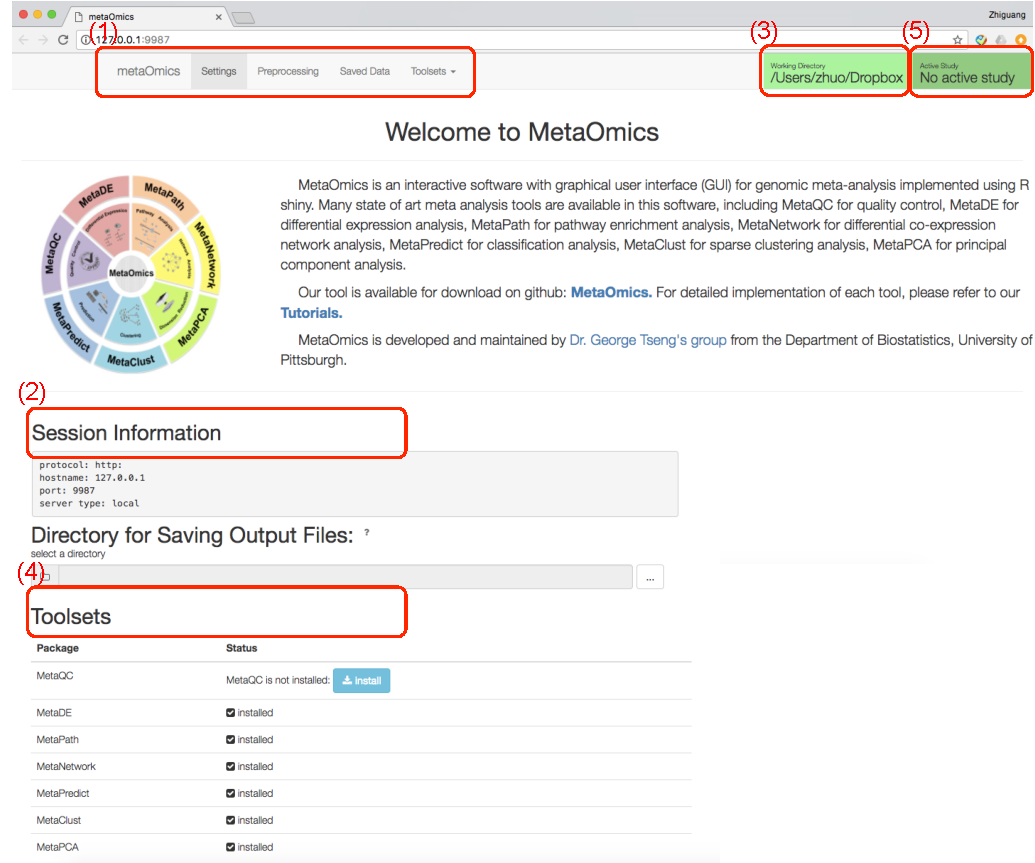
\includegraphics[scale=0.9]{./figure/preprocessing/GUIsetting}
\caption{MetaOmics software suite GUI setting page}
\label{fig:GUIsetting}
\end{center}
\end{figure}


\subsection{Question and bug report}

If you encounter errors or bugs, please report to maintainer Tianzhou Ma $<$\url{tim28@pitt.edu}$>$.


 
 
\input{content/prepareData.tex} 
 
\section{Toolsets}
\subsection{MetaQC}
For MetaQC, we used prostate cancer datasets with 8 datasets.
??Decide if we need more description here??

\subsubsection{Merging}

The datasets from all the 8 studies (uploaded in ``Preprocessing" step and named as ``p1.csv", ``p2.csv", etc.) should be merged before implementing MetaQC tool (Figure \ref{fig:merge}). The genes with low mean or low variance were filtered out (by default, the lowest 30th percentiles). Detailed information can be found in the ``preproc" package in the metaOmics software suite (\url{https://github.com/metaOmic/preproc}).

\begin{figure}[H]
\begin{center}
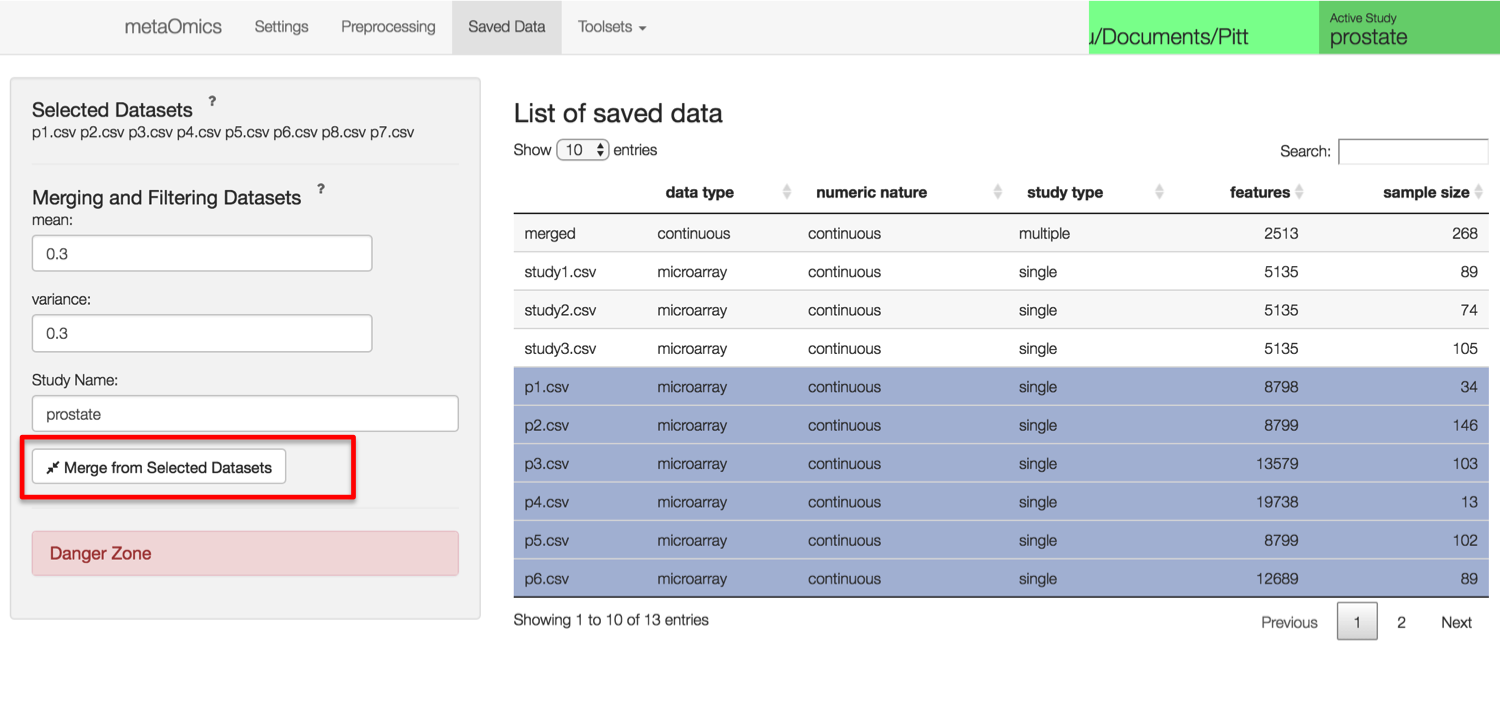
\includegraphics[scale=0.4]{./figure/metaQC/merge2}
\caption{Merging data for meta-analysis}
\label{fig:merge}
\end{center}
\end{figure}

\subsubsection{MetaQC analysis}

After opening the MetaQC page, as shown in Figure \ref{fig:MetaQCmainpage}, there are 2 tabs on the left of the page (``Options" and ``Advanced Options"). We generally suggest users not to change any parameter setting in the ``Advanced Options" unless users know the underlying methodology well. 

\begin{figure}[H]
\begin{center}
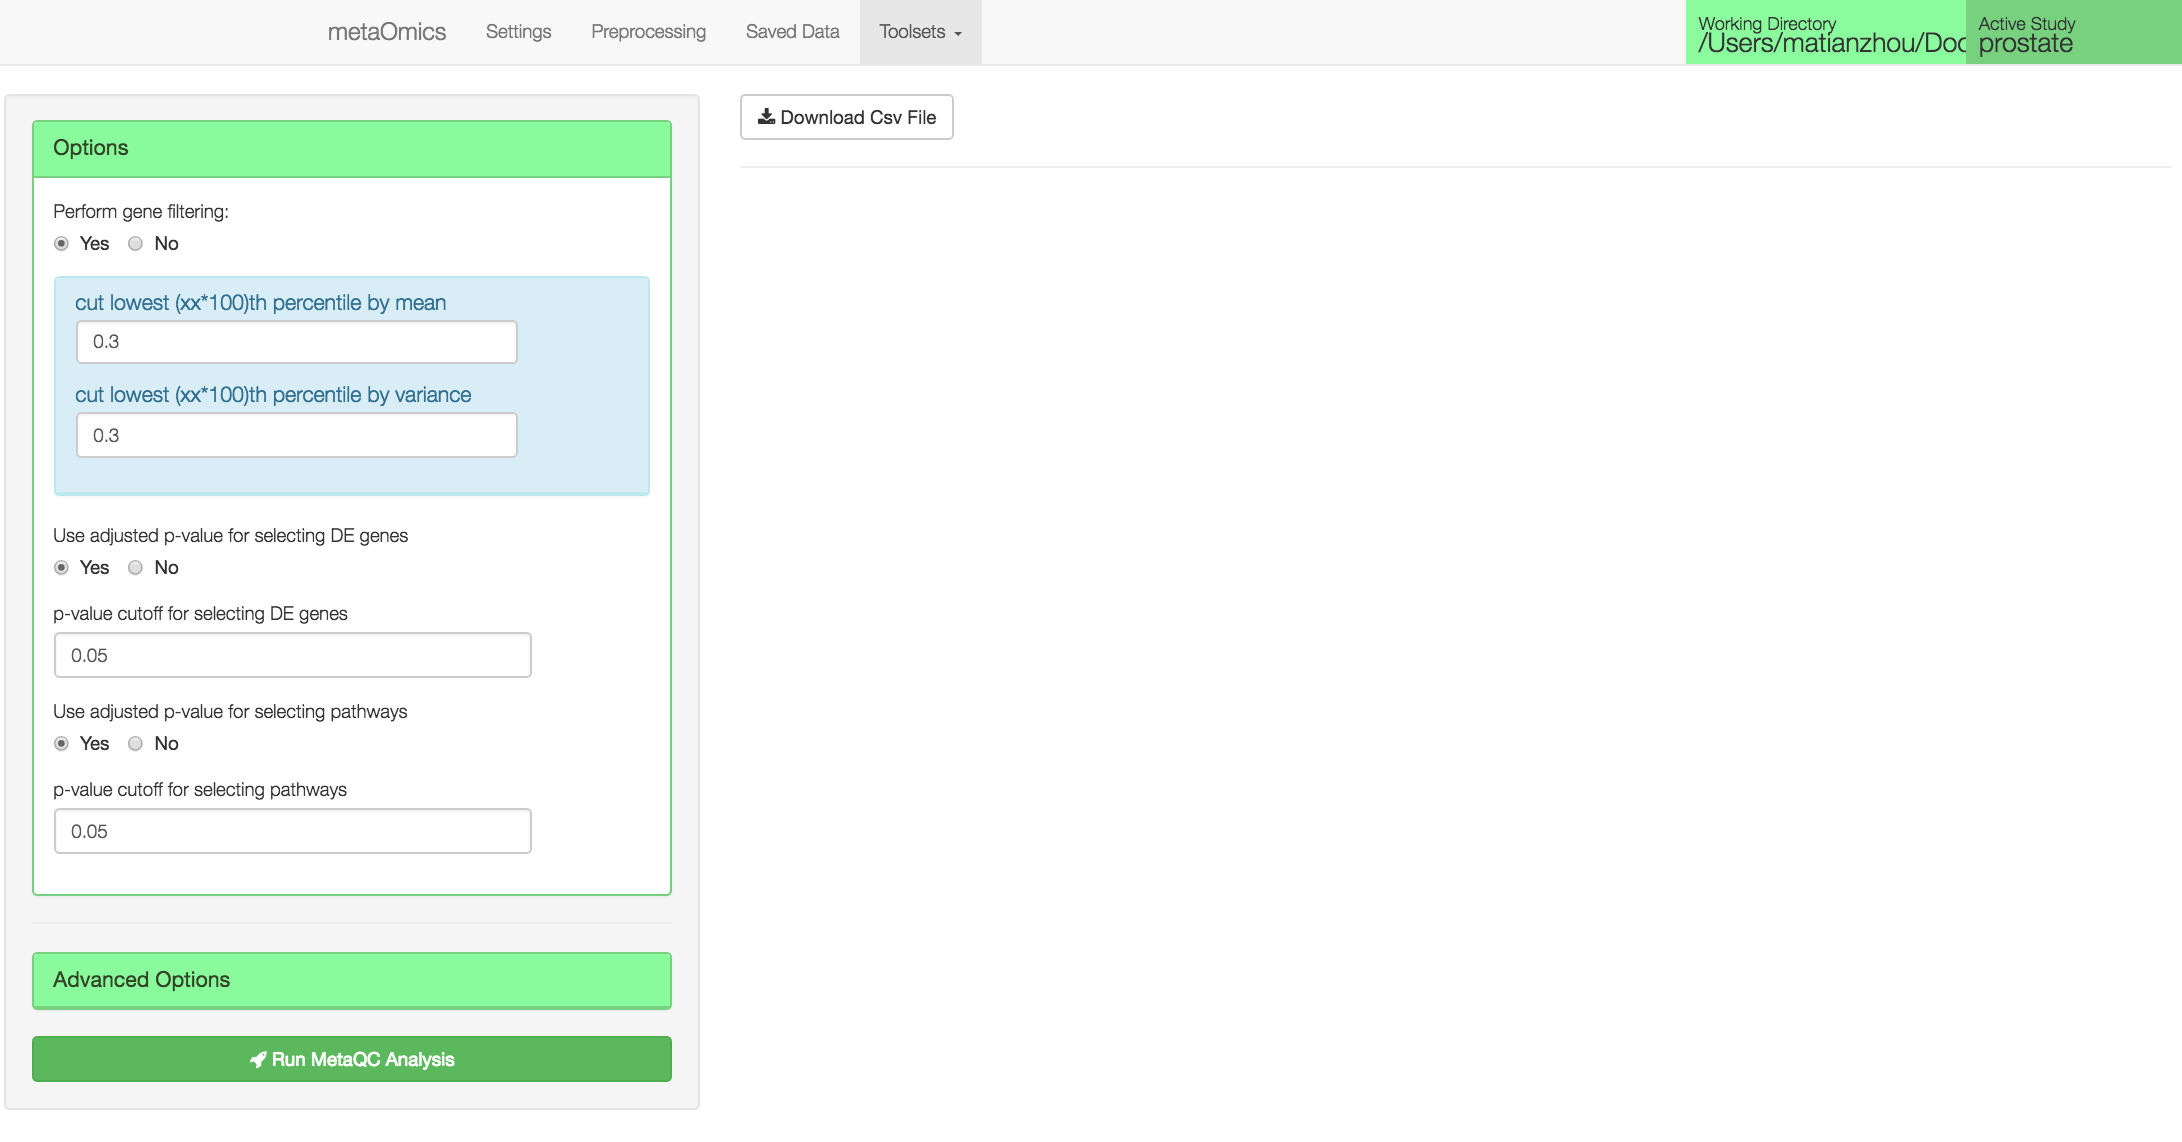
\includegraphics[scale=0.5]{./figure/metaQC/MetaQCmainpage}
\caption{Homepage of MetaQC}
\label{fig:MetaQCmainpage}
\end{center}
\end{figure}

For the current dataset, we already performed filtering while merging the 8 studies so we do not further filtered genes here and chose  ``No" for gene filtering (Figure \ref{fig:option1}). Moreover, MetaQC method requires users to choose a cutoff to decide significant DE genes and a cutoff to decide significantly enriched pathways, there are four options available, i.e. p-value cutoff for selecting DE genes, whether to use adjusted p-value or selecting DE genes, p-value cutoff for selecting pathways, whether to use adjusted p-value or selecting pathways. These options can be tuned depending on the overall signal of the datasets. Here, we use the defaults as determined by the prostate data.   

\begin{figure}[H]
\begin{center}
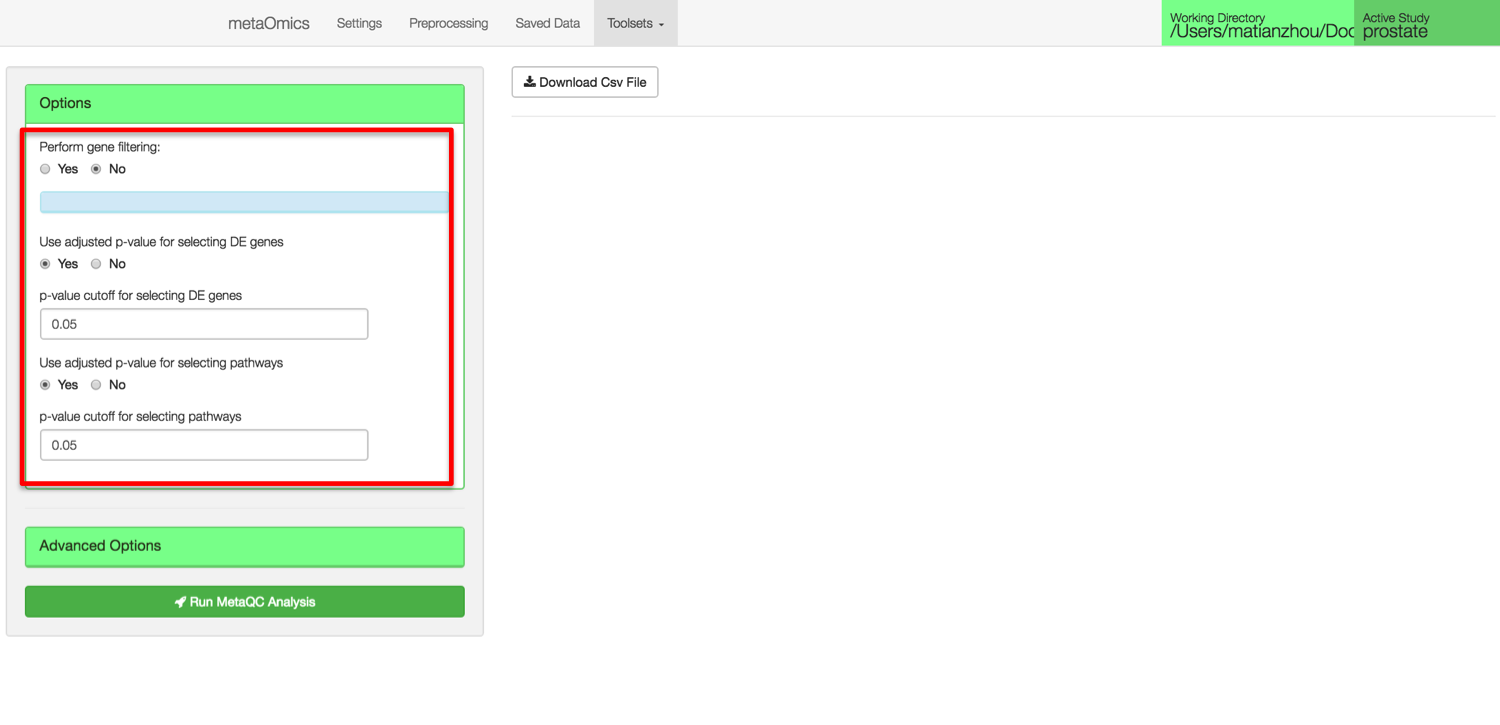
\includegraphics[scale=0.5]{./figure/metaQC/option1}
\caption{MetaQC Options}
\label{fig:option1}
\end{center}
\end{figure}

** Optionally, we can click on ``Advanced Options", choose ``min pathway size" and ``max pathway size" to include only pathways of reasonable size. We suggest 100 permutations is sufficient, and generally do not recommend users to change the number of permutations here (Figure \ref{fig:option2}). 

\begin{figure}[H]
\begin{center}
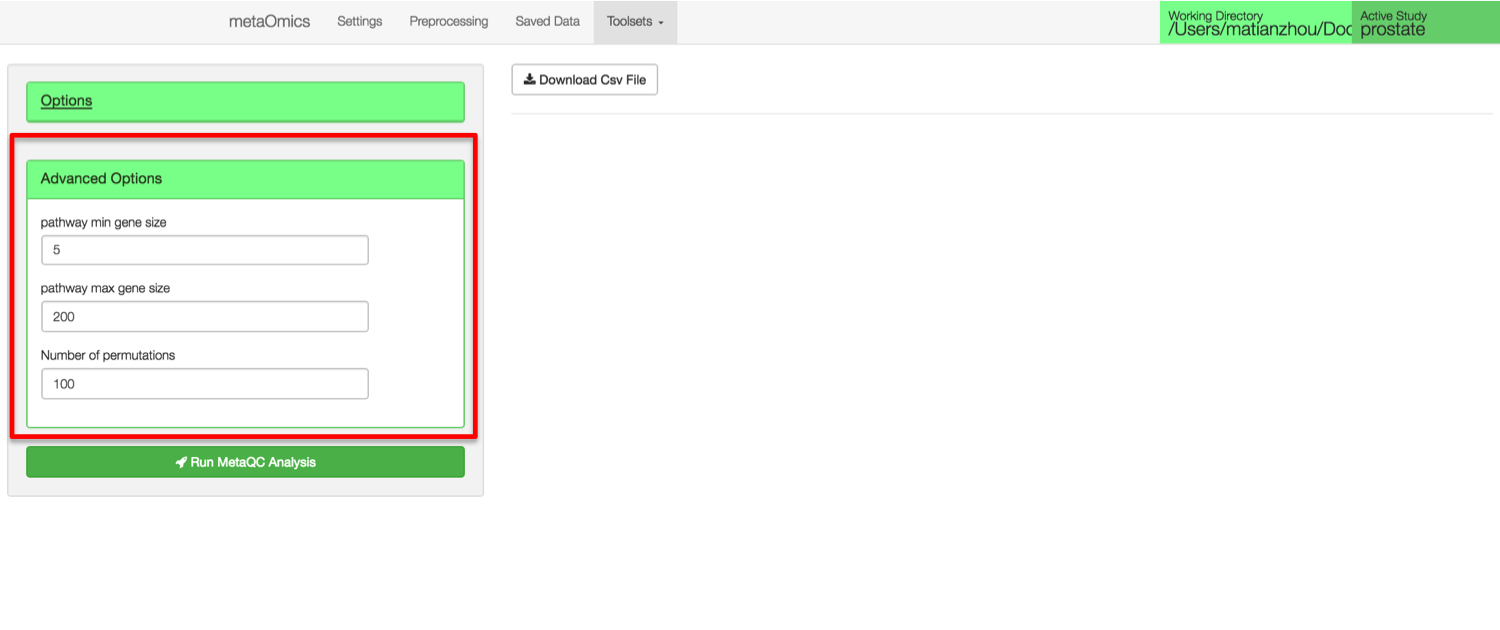
\includegraphics[scale=0.5]{./figure/metaQC/option2}
\caption{MetaQC Advanced Options}
\label{fig:option2}
\end{center}
\end{figure}

After we click on ``Run", we will see a summary table of MetaQC generated on the right of the page as shown in Figure \ref{fig:result}. The table includes seven columns, with the first six columns corresponding to the six quantitative quality control measures of all studies (a larger value indicates a better quality) and the seventh column is the rank summary statistics of all the six quality measures (a lower rank indicates a better quality). Users can download the full table as a csv file by clicking on ``Download Csv File". In addition to the tabular results, the tool also generated a PCA biplot from the six quality control measures, where the circled number is the study index and arrows indicate different measures (Figure \ref{fig:result}). Both tabular summary and biplot are automatically saved to the current working directory. 

\begin{figure}[H]
\begin{center}
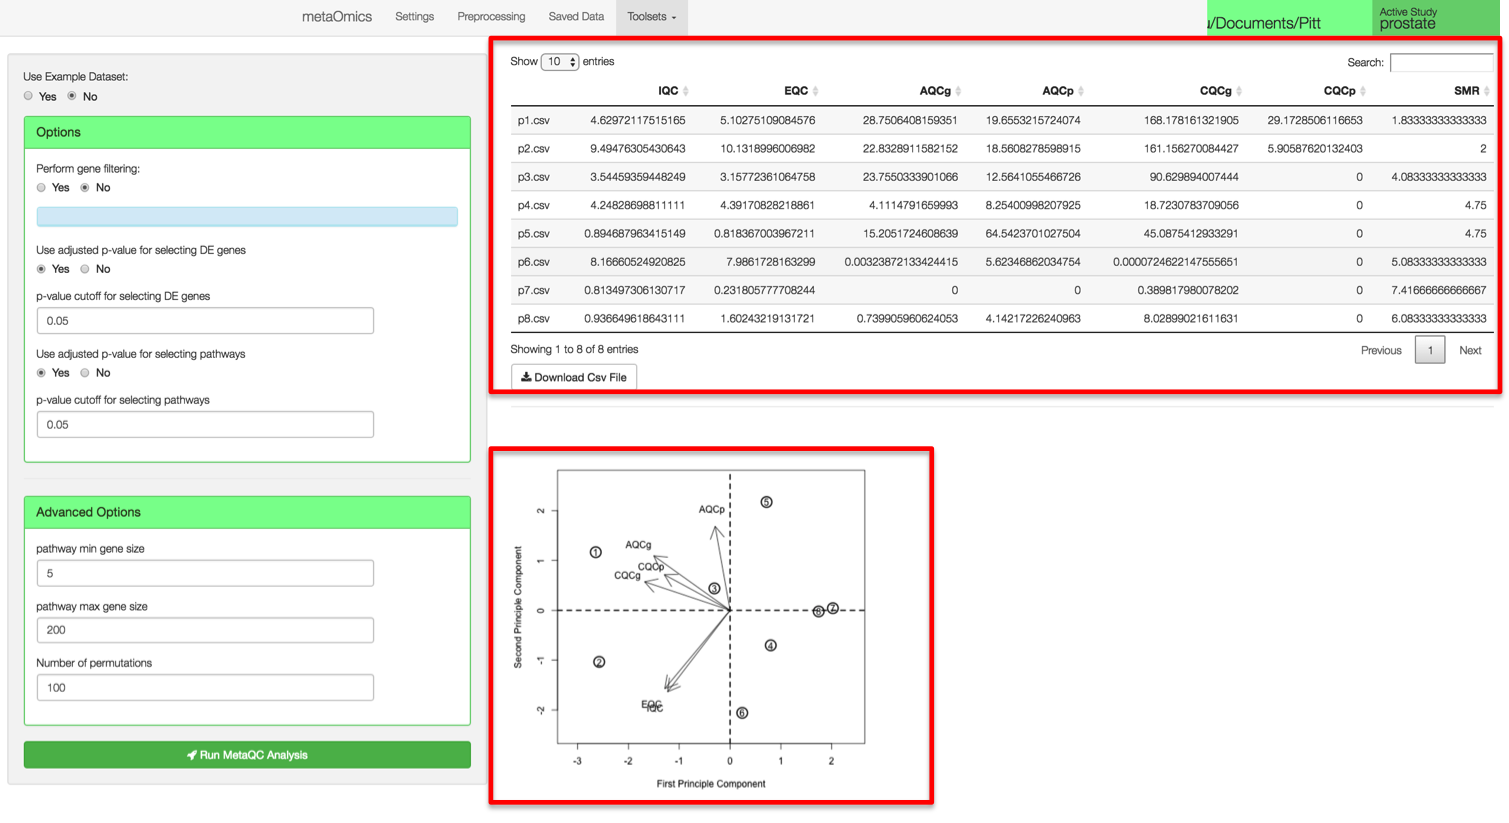
\includegraphics[scale=0.5]{./figure/metaQC/result}
\caption{MetaQC results: summary table and PCA biplot}
\label{fig:result}
\end{center}
\end{figure}


 
\subsection{MetaDE}

MetaDE package implements 12 major meta-analysis methods for differential expression analysis falling into 3 main categories: combining p-values, combining effect sizes and others (e.g. combining ranks, etc.). Depending on the types of outcome, the package can perform two class comparisons, multi-class comparison, association with continuous or survival outcome. The package allows the input of either microarray (continuous intensity) and/or RNA-seq data (count) for individual study analysis. 
The R package for MetaDE module can be found \url{https://github.com/metaOmics/MetaDE}.
After obtaining DE genes from meta-analysis, 
users can further perform pathway enrichment analysis based on the declared DE genes.
In the two subsections below we will go over how to perform (1) meta-analysis and (2) pathway enrichment analysis based on (1).


\subsubsection{Procedure of Meta-analysis for differential expression}

\begin{figure}[H]
\begin{center}
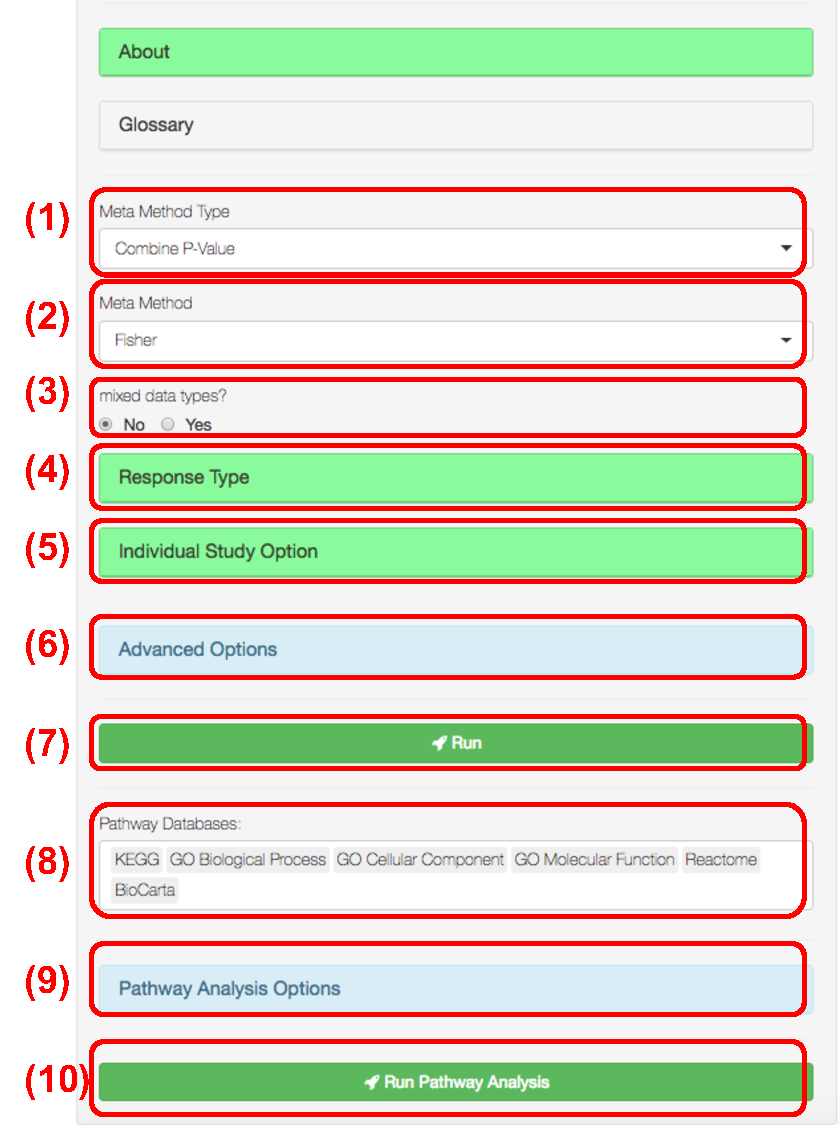
\includegraphics[scale=0.5]{./figure/metaDE/metaDEoption.pdf}
\caption{``MetaDE" options}
\label{fig:MetaDEoption}
\end{center}
\end{figure}

In Figure~\ref{fig:MetaDEoption},
{\color{red} Red boxes (1) - (7)} are the steps to tuning parameters and run meta-analysis.
A detailed list of all options available for the package can be found at the end of this subsection. 

\begin{steps}
\item \textbf{Choose the type of meta-analysis methods:}
There are three types of meta-analysis to choose:
combining p-values, combining effect size and others.

\item \textbf{Choose a meta-analysis method:}
\begin{itemize}
\item For ``combining p-values" category,
users can choose from ``Fisher", ``AW-Fisher", ``maxP", ``minP", ``roP" and ``Stouffer",
where some of them have the one-sided corrected versions.

\item For ``combining effect size" category,
users can choose from ``FEM" and ``REM",
where ``REM" has choice of six analytical algorithms for implementation.

\item For ``others",
there are three rank-based method (PR, SR and rankProd) and minMCC for multi-class meta-analysis.
To choose from the overwhelmingly many meta-analysis methods,
we follow \cite{chang2013meta} and mark * for top performing methods AW-Fisher, REM (HO option) and roP as recommendation for users.
\end{itemize}

\item \textbf{Mixed data type:}
If this option is selected,
MetaDE will allow partial studies with count data from RNA-seq and remaining studies with continuous intensities from microarray.

\item \textbf{Choose the response type:}
Under the drop-down menu,
users can specify types of outcome (response) variable to be two-class, continuous, multi-class or survival.
By choosing ``two class comparison",
users can specify the group label name for the Label Attribute (from the column names of your clinical data).
Then for group label (a factor of at least two levels),
specify the name for the ``Control Label" and ``Experimental Label", respectively.
For the other types, only group label name is needed.

\item \textbf{Choose Study Design for individual study:}
\begin{itemize}
\item Individual data type can be either discrete (count) or continuous.
\item Under drop-down menu ``Setting Individual Study method", user can specify  individual study method according to individual data type.
For continuous data (e.g. microarray), available options include LIMMA (default method) and SAM.
For discrete data (e.g. RNA-seq count), available options include edgeR, DESeq2 and voom.
\item The users can also specify whether each study is paired design or not.
\end{itemize}

\item \textbf{Advanced Options}
\begin{itemize}
\item Use complete options: other uncommonly used options will become available. Again, this is not suggested if you are not familiar with the method.
\item Parametric: if No is selected, permutation will be performed instead of parametric closed form solution.
\item Covariate: indicate if any covariate will be adjusted.
\item Alternative Hypothesis: two-sided or one-sided.
\end{itemize}

\item \textbf{Run:}
Once all the above options are specified, users can click on ``Run" button to perform MetaDE analysis

\end{steps}


\subsubsection{Results of Meta-analysis for differential expression}

For the MetaDE model, we used multi-study leukemia gene expression data as example.
After performing merging of the three datasets and filter 50\% genes by mean and 50\% by variance, 1283 genes remained.
In this example we only compare two phenotypes: inv(16) and t(15;17).
Two main outputs from the first ``meta differential analysis" step in the procedure are shown in Figure \ref{fig:MetaDEresult1}. 
Heatmap of DE genes is drawn on top after specifying the FDR cutoff for selection of DE genes and clicking on ``Plot DE Genes Heatmap". 
The ``image size" can be adjusted by dragging the scroll bar. 
In the heatmap, rows refer to DE genes selected, columns refer to samples, solid white lines are used to separate different studies and the dashed white lines are used to separate groups. 
Colors of the cells correspond to scaled expression level as indicated in the color key below. 
For the results generated by ``AW-Fisher", there is one additional column of cross-study weight distribution on the left end of the heatmap and the genes in the heatmap are sorted by their weight distribution.
Summary of meta analysis results is on bottom, 
including information of individual test statistics, individual study p-value, meta-analysis p-value, FDR, etc. 


\begin{figure}[H]
\begin{center}
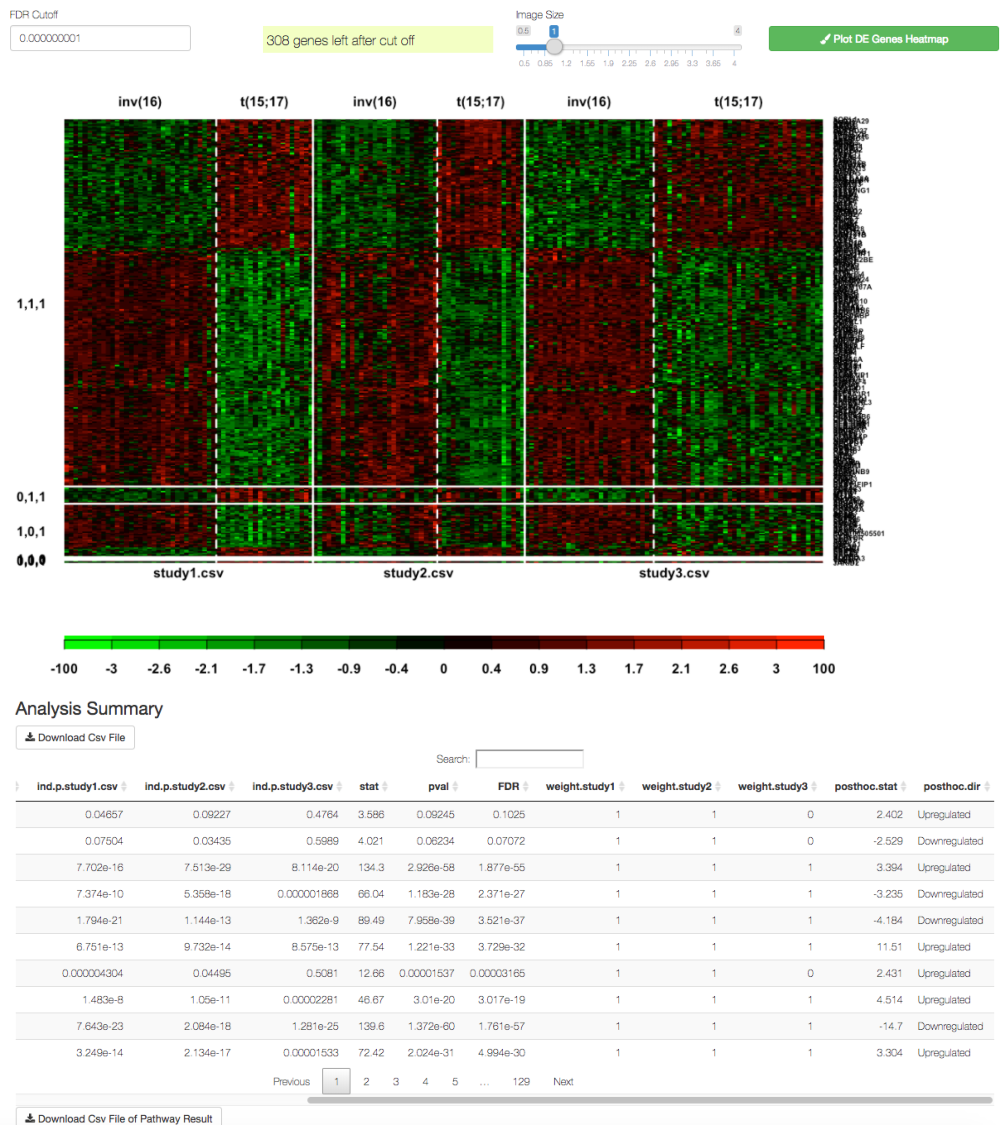
\includegraphics[scale=0.9]{./figure/metaDE/metaDEresult.pdf}
\caption{``MetaDE" Results}
\label{fig:MetaDEresult1}
\end{center}
\end{figure}

\subsubsection{Procedure of downstream pathway analysis}
Users can then perform pathway enrichment analysis on the declared DE genes from the previous step, 
which can be achieved in {\color{red} Red boxes (8) - (10)} in Figure~\ref{fig:MetaDEoption}.
Procedure is ruled out as below.

\begin{steps}
\item \textbf{Choose the pathway database:}
Users can select from 25 available pathway databases to perform the pathway enrichment analysis. 

\item \textbf{Choose the pathway enrichment method and the pathway size range:}
In this step users can choose pathway enrichment options with Kolmogorov-Smirnov (KS) test as default option,
or Fisher's exact test by specifying number of input genes for pathway analysis.
For Fisher's exact test, the input genes can be obtained by either specifying a MetaDE p-value cutoff, or specifying number of top DE genes.
Users can also specify the minimum/maximum gene size of pathways to be included for pathway enrichment analysis.

\item \textbf{Run:}
Once all the above options are specified, users can click on ``Run Pathway analysis" button to perform pathway enrichment analysis.

\end{steps}


\subsubsection{Result of downstream pathway analysis}

The result for downstream pathway analysis  is tabulated in Figure \ref{fig:MetaDEresult2}. 
The summary includes the pathway names, the corresponding enrichment p-value and FDR. 
In addition to the results shown in the browser, 
users can download the result by clicking on "Download Csv File" on the top left of the summary table. 

\begin{figure}[H]
\begin{center}
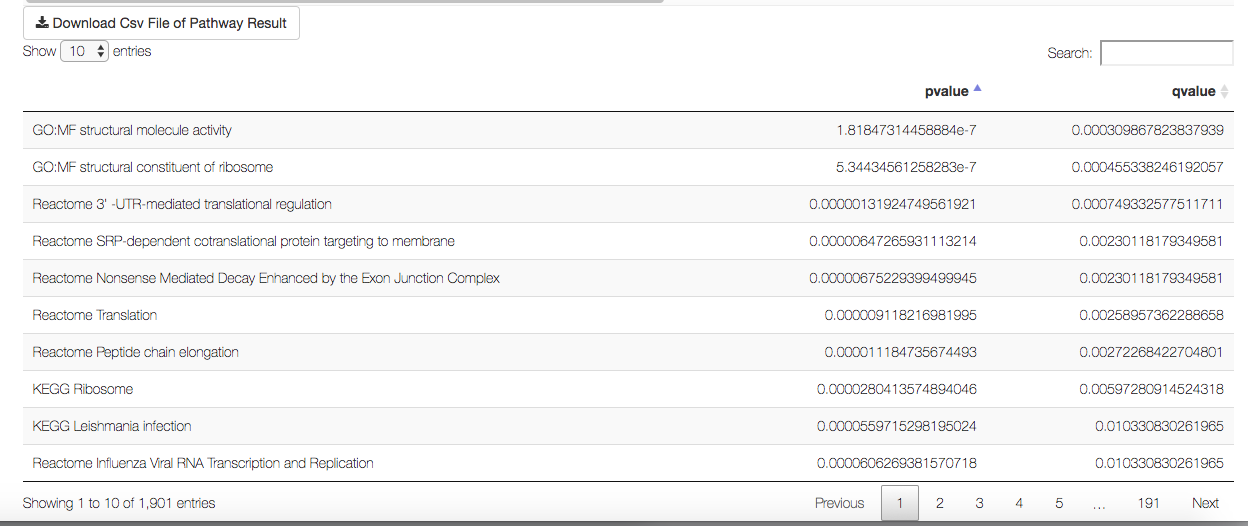
\includegraphics[scale=0.4]{./figure/metaDE/MetaDE_pathway.png}
\caption{Downstream pathway analysis based on MetaDE genes}
\label{fig:MetaDEresult2}
\end{center}
\end{figure}


\textbf{Complete List of Options:} 

\begin{enumerate}
  \item Meta Method Type: Combining p-value, Combining effect size, Others.
  \item Meta Method: Fisher, AW-Fisher, FEM, REM, Sum of Rank, Produce of Rank, multi-class correlation, Rank product. 
  \item Mixed data type: selected if both count data and continuous data exist.
  \item Response Type:
   \begin{itemize}
     \item Two class comparison, Multi-class comparison, Continuous outcome, Survival outcome.
     \item Label Attribute: select the label name of the outcome.
     \item Control Label \& Experimental Label: specify the case/control label for two-class comparison.
    \end{itemize}
   \item Individual Study Option:
     \begin{itemize}
     \item Setting individual study method
     \item Setting individual study paired option
    \end{itemize} 
   \item Advanced Option (**Optional):
     \begin{itemize}
      \item Use complete options
      \item Parametric
      \item Covariate
      \item Alternative hypothesis
    \end{itemize} 
    \item Run
    \item Pathway Databases
    \item Pathway Analysis Option:
         \begin{itemize}
      \item Pathway enrichment method
      \item Pathway min gene size
      \item Pathway max gene size
    \end{itemize} 
    \item Run Pathway Analysis
\end{enumerate}



 
\subsection{MetaPath}

In MetaDE package,
following the detection of biomarkers, pathway analysis (a.k.a. gene set enrichment analysis) is usually performed for functional annotation and biological interpretation. 
Beyond that, the MetaPath module provides two advanced meta-analytic pathway analysis tools: 
Comparative Pathway Integrator (CPI) and Meta-Analysis for Pathway Enrichment (MAPE) (Shen et al., 2010; Fang et al., 2017). 
Pathway clustering with statistically valid text mining is included in the package to reduce pathway redundancy to condense knowledge and increase interpretability of clustering results. 
The R package for MetaPath module can be found \url{https://github.com/metaOmics/MetaPath}.

\subsubsection{Procedure}
The MetaPath package requires the input of raw expression data as in MetaDE. 
There are three major steps to implement the package: pathway analysis, pathway clustering diagnostics and pathway clustering with text mining. 
As shown in Figure \ref{fig:MetaPathoption}, there are 9 major options that need to be specified to implement the package.
Detailed list of all options available for the package can be found at the end of this subsection. 


\begin{figure}[H]
\begin{center}
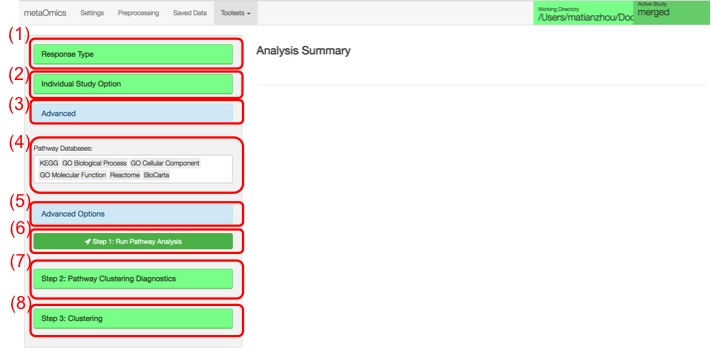
\includegraphics[scale=0.5]{./figure/metaPath/metaPathoption.pdf}
\caption{``MetaPath" options}
\label{fig:MetaPathoption}
\end{center}
\end{figure}

\begin{steps}
\item \textbf{Setup pathway analysis parameters:}
Users need to specify {\color{red}(1) } whether the input gene expression profile is mixed of continuous data and discrete data;
{\color{red}(2)} response type, case/control labels (similar to MetaDE);
{\color{red}(3)} individual study option (similar to MetaDE);
{\color{red}(4)} advanced options including whether to adjust for covariates or the direction of hypothesis testing;.
In {\color{red}(5)}, users can select from 25 available pathway databases for the enrichment analysis.
In {\color{red}(6)}, users can select MetaPath method (either CPI or MAPE).
By default, the ``CPI" approach is used, otherwise ``MAPE" approach can also be used. Other options include pathway enrichment method (the Fisher's exact test or KS test), the minimum and maximum pathway size. If ``Fisher's exact test" is chosen for the enrichment method, users need to further specify the criteria for selection of DE genes, e.g. the number of top ranked genes. On the other hand, if ``KS test" is chosen, one needs to further specify whether to use permutation to obtain enrichment p-value. 

\item \textbf{Run Pathway Analysis:}
\label{step:metaPath1}
Once the above options are specified, users can click on {\color{red}(7)}, ``Run Pathway Analysis".

\textbf{Pathway clustering diagnostics:} 
\label{step:metaPath2}
From the previous step (Step~\ref{step:metaPath2}), users can choose the top enriched pathways for further clustering. 
One can expand the drop-down menu and use FDR cutoff to choose top pathways and click on {\color{red}(8)}, ``Pathway clustering diagnostics" to implement the second step.

\textbf{Pathway clustering with text mining:} 
\label{step:metaPath3}
From the previous step (Step~\ref{step:metaPath3}), users can determine the optimal number of clusters in the pool of pathways selected. 
Now, one can specify the number of clusters and click on {\color{red}(9)} ``Get clustering result" to implement the third step. 
Note that you may not want to select too large $K$ since you wish to have a certain amount of pathways in each cluster for the validity of text mining algorithm. 
We generally suggest users to specify $K$ no larger than 7 for fewer than 100 pathways. 
\end{steps}





\textbf{Complete List of Options:} 

\begin{enumerate}
  \item mixed data types: whether the input data is a mixture of count data and continuous data.
  \item Response Type:
   \begin{itemize}
     \item Two class comparison, Multi-class comparison, Continuous outcome, Survival outcome.
     \item Label Attribute: select the label name of the outcome.
     \item Control Label \& Experimental Label: specify the case/control label for two-class comparison.
    \end{itemize}
   \item Individual Study Option:
     \begin{itemize}
     \item Setting individual study method
     \item Setting individual study paired option
    \end{itemize} 
   \item Advanced Option (**Optional):
     \begin{itemize}
      \item Covariate
      \item Alternative hypothesis
    \end{itemize} 
    \item Pathway Databases
    \item Pathway Analysis Option:
         \begin{itemize}
       \item Software
      \item Pathway enrichment method
      \item Pathway min gene size
      \item Pathway max gene size
    \end{itemize} 
    \item Run Pathway Analysis
    \item Pathway Clustering Diagnostics
    \item Get Clustering Result
\end{enumerate}


\subsubsection{Results}

\begin{figure}[H]
\begin{center}
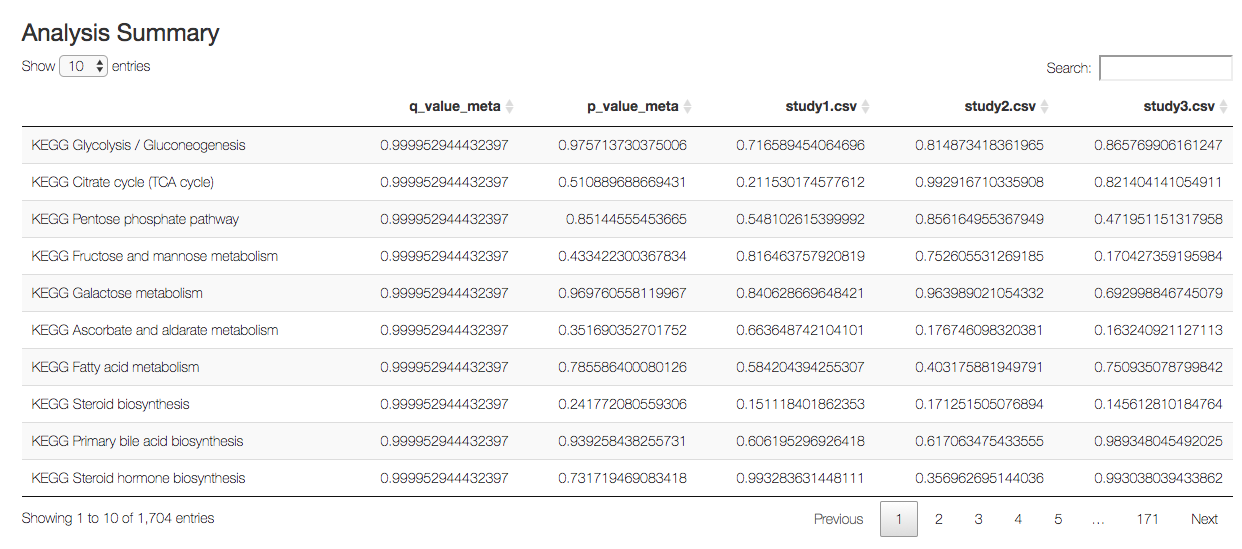
\includegraphics[scale=0.4]{./figure/metaPath/metaPathresult1.png}
\caption{``MetaPath" Results (1)}
\label{fig:MetaPathresult1}
\end{center}
\end{figure}

The input dataset is same as the input for MetaDE module.
We used multi-study leukemia gene expression data as example.
After performing merging of the three datasets and filter 50\% genes by mean and 50\% by variance, 1283 genes remained.
In this example we only compare two phenotypes: inv(16) and t(15;17).

After the Step~\ref{step:metaPath1} is finished, a summary table was generated as shown in Figure~\ref{fig:MetaPathresult1} (based on the default CPI method). The ``Analysis Summary" includes the analysis results of all pathways, including individual study association analysis p-value, meta pathway analysis p-value/FDR, etc. Users can search the gene name in the ``Search" bar, and the full table is automatically saved in the working directory specified before.  

\begin{figure}[H]
\begin{center}
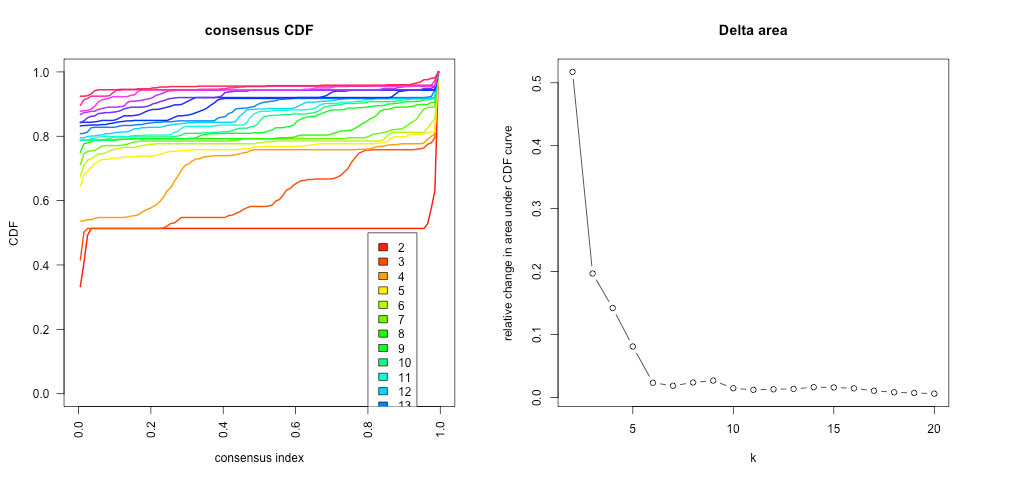
\includegraphics[scale=0.5]{./figure/metaPath/metaPathresult2.png}
\caption{``MetaPath" Results (2)}
\label{fig:MetaPathresult2}
\end{center}
\end{figure}

After the ``Pathway Cluster Diagnostics" step is finished, we will see two plots generated on the right panel (Figure \ref{fig:MetaPathresult2}): consensus CDF and Delta area plots, both from the ``ConsensusClusterPlus" package. The CDF of the consensus matrix for each $K$ (indicated by colors) is estimated by a histogram of 100 bins. The CDF
reaches an approximate maximum, thus consensus and cluster confidence is at a maximum at this $K$. The delta area shows the relative change in area under the CDF curve comparing $K$ and $K - 1$, thus allows users to determine the determine $K$ at which there is no appreciable increase in CDF. Both plots assist users in finding the optimal number of clusters $K$ and you may refer to (Monti et al., 2003) for more detailed interpretation of the two plots. In the demo example, $K=6$ have large enough CDF, is thus chosen (though $K=7$ captures more, we only have 38 pathways here). 

\begin{figure}[H]
\begin{center}
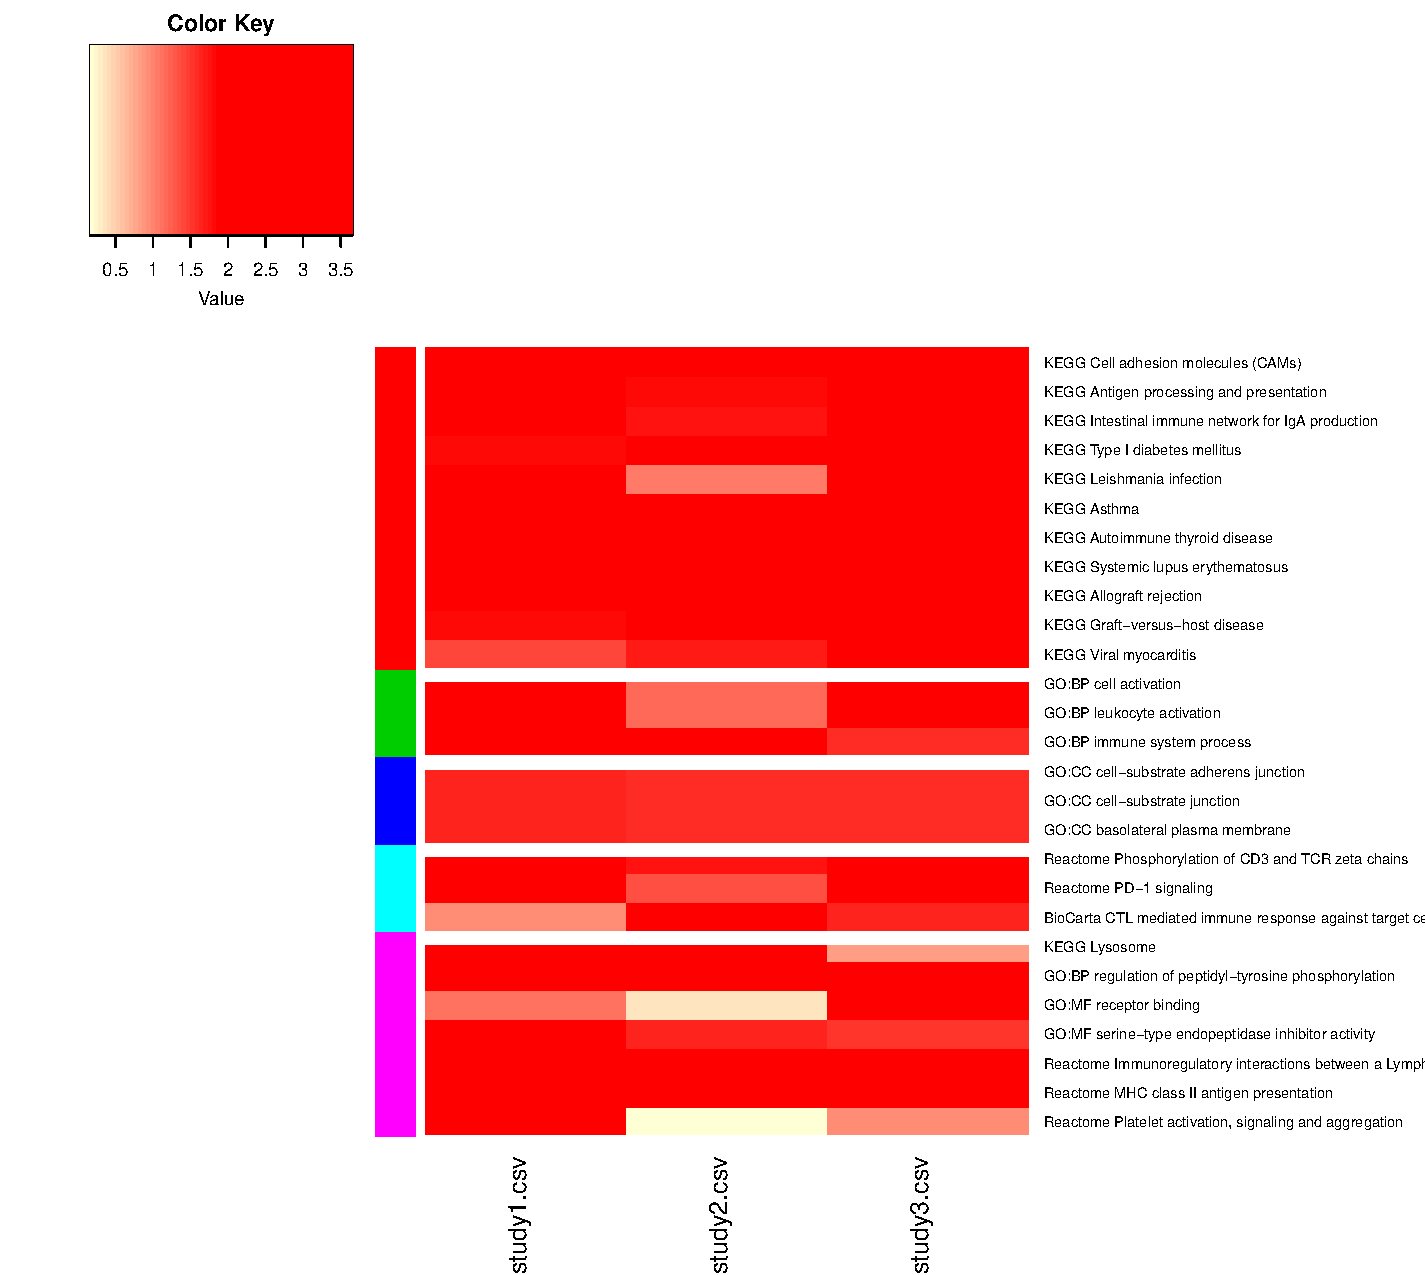
\includegraphics[scale=0.6]{./figure/metaPath/Heatmap_clusters_all.pdf}
\caption{``MetaPath" Results (3)}
\label{fig:MetaPathresult3}
\end{center}
\end{figure}


The heatmap in Figure~\ref{fig:MetaPathresult3} shows the -log10 transformed p-value of enrichment analysis in each study from \ref{step:metaPath1}. 
Studies are on columns and the selected pathways are on rows, red means more enriched. The pathways are sorted by the pathway cluster as indicated by the colors on the left side of the heatmap. 
In addition, 
the key words of each cluster of pathways are extracted and analyzed by a built-in text mining algorithm and one file named ``Clustering\textunderscore Summary.csv" is saved to the working directory which shows a summary of the text mining result. 



 
\subsection{MetaClust}
By clicking toolsets and then metaClust,
users are directed to metaClust home page as Figure~\ref{fig:metaClustHome}.
MetaClust \citep{huo2016meta} aims to perform sample clustering analysis combining multiple transcriptomic studies.
By integrate information from multiple studies of similar biological purposes,
MetaClust can identify an unified intrinsic gene sets among all studies, perform weighted clustering analysis using these common intrinsic gene sets,
match the clustering pattern across studies to define disease subtype/cluster type.
The resulting clustering from meta-analysis is more robust and accurate than single study analysis.
The R package for MetaClust module can be found \url{https://github.com/metaOmics/MetaSparseKmeans}.


\begin{figure}[H]
\begin{center}
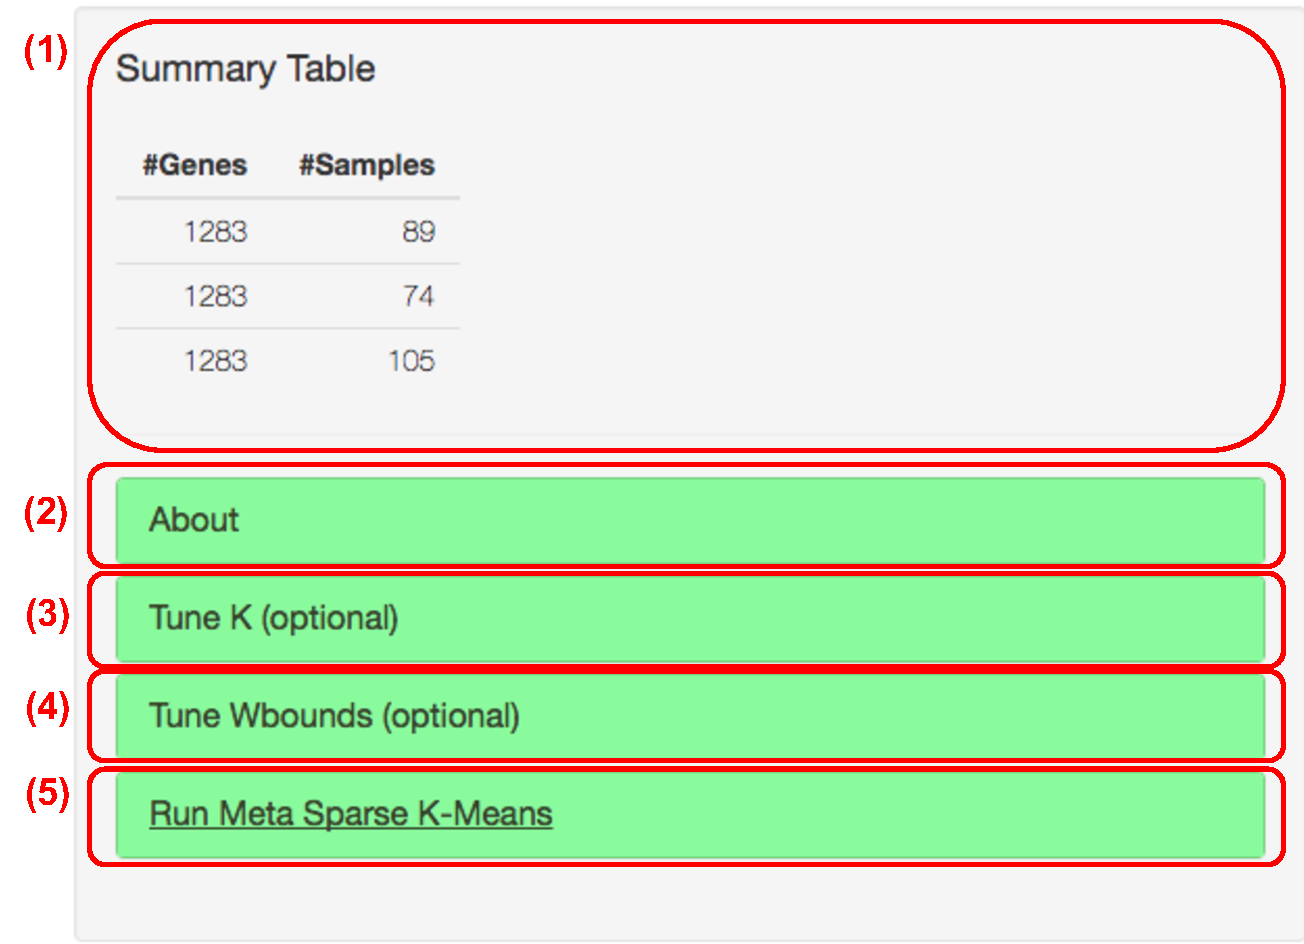
\includegraphics[scale=0.4]{./figure/metaClust/metaClustHome.pdf}
\caption{MetaClust home page}
\label{fig:metaClustHome}
\end{center}
\end{figure}

\subsubsection{Procedure}

Figure~\ref{fig:metaClustHome} shows the home page of MetaClust.
On the top left panel users can see data summary Table (at position {\color{red} (1)}).
Below there are 4 tabs. 
About tab (at position {\color{red} (2)}) includes basic introduction of MetaClust.
Starting with multiple studies, 
we could run MetaSparseKmeans (at position {\color{red} (5)}) with pre-specified number of clusters (K) and gene selection tuning parameter (Wbounds).
If you are not sure about what are good K and Wbounds, please try Tune K (at position {\color{red} (3)}) and Tune Wbounds (at position {\color{red} (4)}) panel.

\begin{steps}

\item \textbf{Tune K:} 

\begin{figure}[H]
\begin{center}
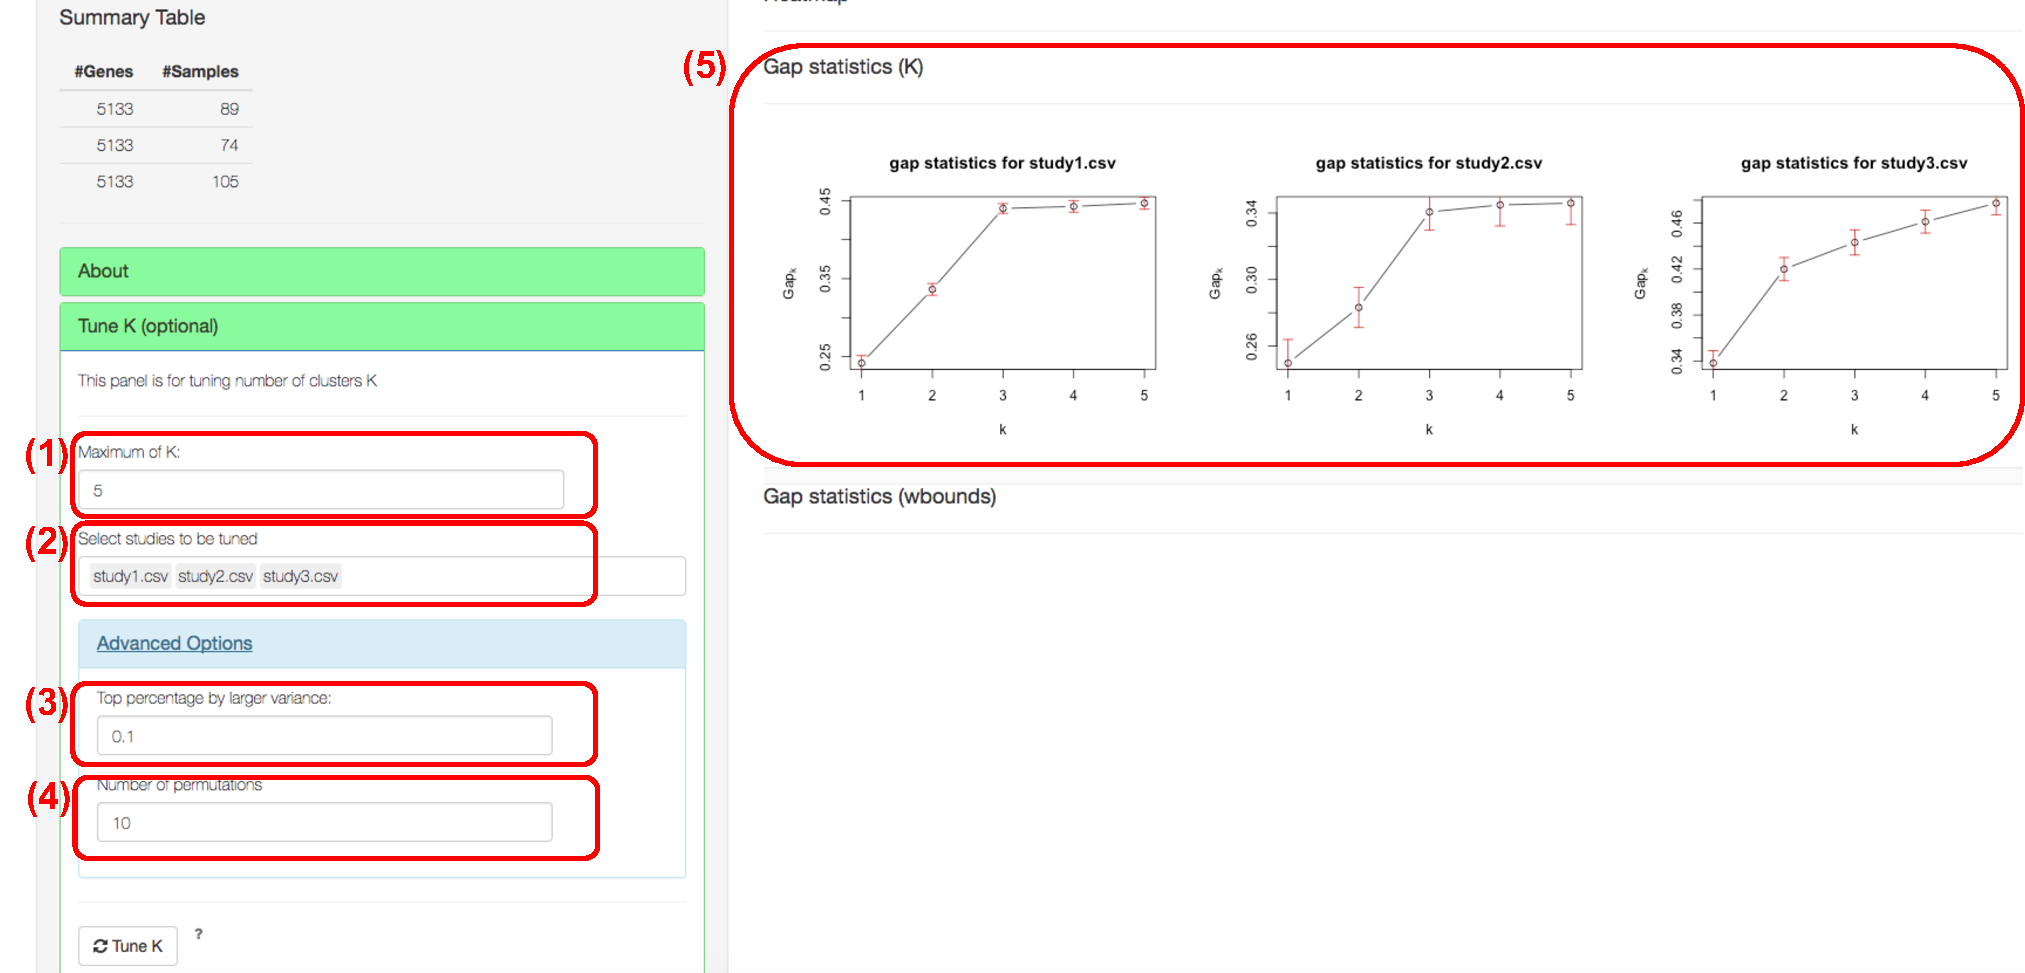
\includegraphics[scale=0.5]{./figure/metaClust/tuneK.pdf}
\caption{Tuning parameter selection for number of clusters}
\label{fig:metaClusttuneK}
\end{center}
\end{figure}

If the users are not sure what is number of clusters,
they can start to use the Tune K panel as in Figure~\ref{fig:metaClusttuneK}.
Gap statistics will be used to get optimal K for each individual study.
Users need to specify maximum number of K (at position {\color{red} (1)}), which the algorithm will search number of studies from 1 to K.
Studies to be tuned can be selected (at position {\color{red} (4)}).
In advanced options, users can further specify number of top variance genes to be included and number of permutations.
But if users don't know the algorithm, please leave them as default.
Top percentage p\% by larger variance means that we will use top p\% larger variance genes to perform gap statistics (at position {\color{red} (3)}).
Number of permutation is number of bootstrap samples for gap statistics (at position {\color{red} (4)}).
At least 50 bootstrap samples are suggested for a stable result of number of clusters.
By clicking button ``Tune K",
we will obtain gap statistics as in Figure~\ref{fig:metaClusttuneK}.
A good K is selected such that the $\mbox{Gap}_k$ is maximized or stabilized across all studies.
From the figure, K=3 is preferred since the gap statistics from all three studies become flat (at position {\color{red} (5)}).

\item \textbf{Tune Wbounds:} 

Wbounds directly control number of features selected by metaClust.
If the users are not sure what is a good Wbound,
they can start to use the Tune Wbounds panel as in Figure~\ref{fig:metaClusttuneW}.
\begin{figure}[H]
\begin{center}
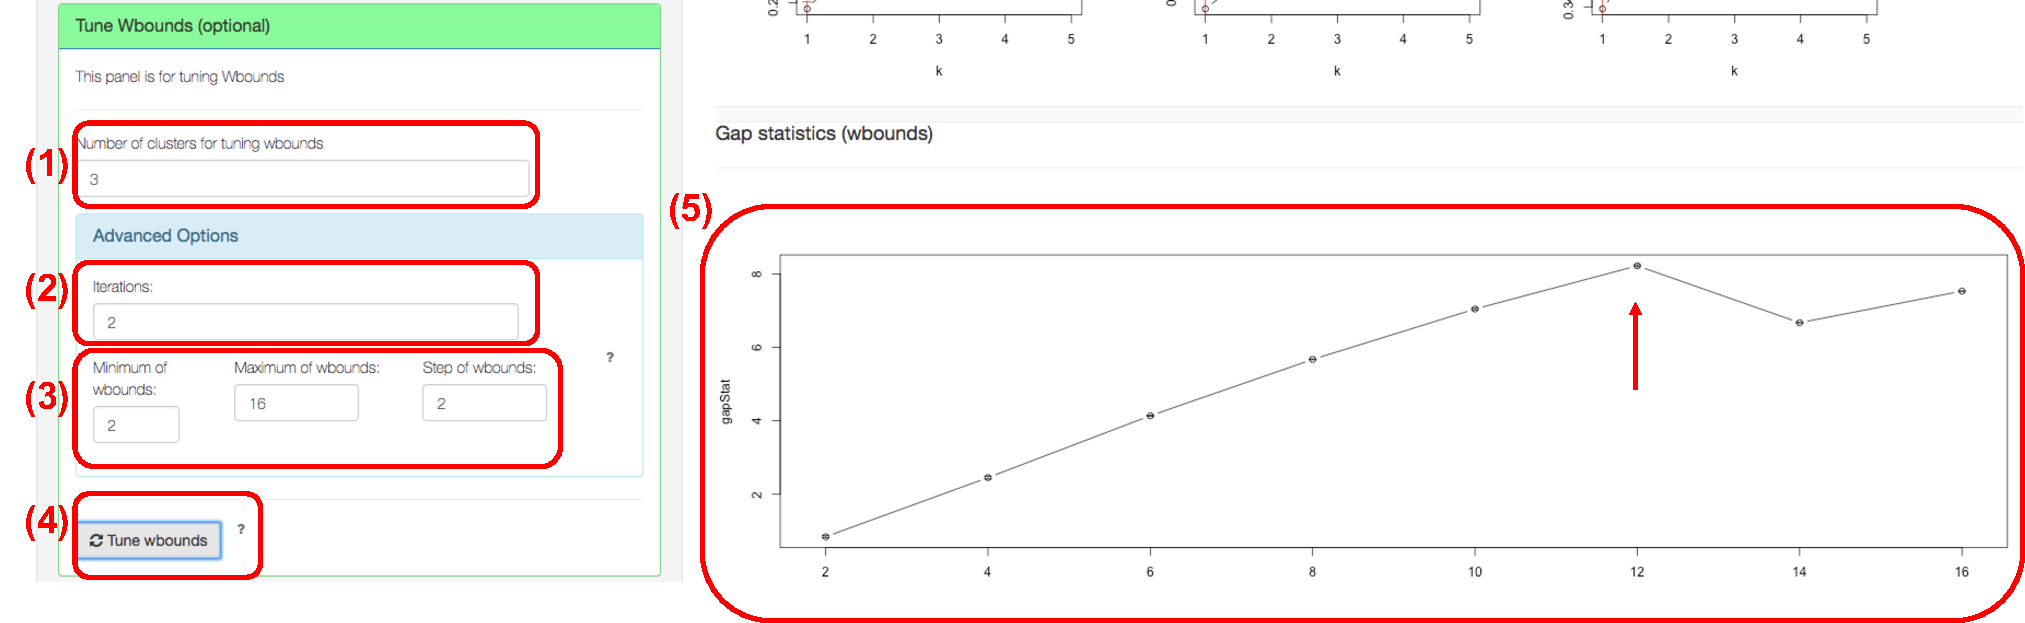
\includegraphics[scale=0.5]{./figure/metaClust/tuneW.pdf}
\caption{Wbound selection}
\label{fig:metaClusttuneW}
\end{center}
\end{figure}
Again,
gap statistics will be used for tuning Wbounds.
Users will specify number of clusters for tuning Wbounds (at position {\color{red} (1)}), which could be obtained from the previous step.
In advanced options, users can further specify number of iterations and the range of candidate Wbounds.
But if users don't know the algorithm, please leave them as default.
Iterations (at position {\color{red} (2)}) is the same thing as number of bootstrap samples for gap statistics.
Users also need to specify the searching space of Wbounds by minimum of Wbounds, maximum of Wbounds and Step of Wbounds (at position {\color{red} (3)}).
After all these steps are set,
user can click on ``Tune Wbounds" button (at position {\color{red} (4)}).
The results will be shown in Figure~\ref{fig:metaClusttuneW}  position {\color{red} (5)}.
Wbound=12 is preferred since the corresponding gap statistics is maximized (where the red arrow indicates).

\item \textbf{Run Meta Sparse K-Means:} 

Under Run Meta Sparse K-Means panel,
user can specify number of clusters (at position {\color{red} (1)}), Wbounds (at position {\color{red} (2)}) and run meta sparse K means (at position {\color{red} (5)}), 
as in Figure~\ref{fig:mskmRes}.
\begin{figure}[H]
\begin{center}
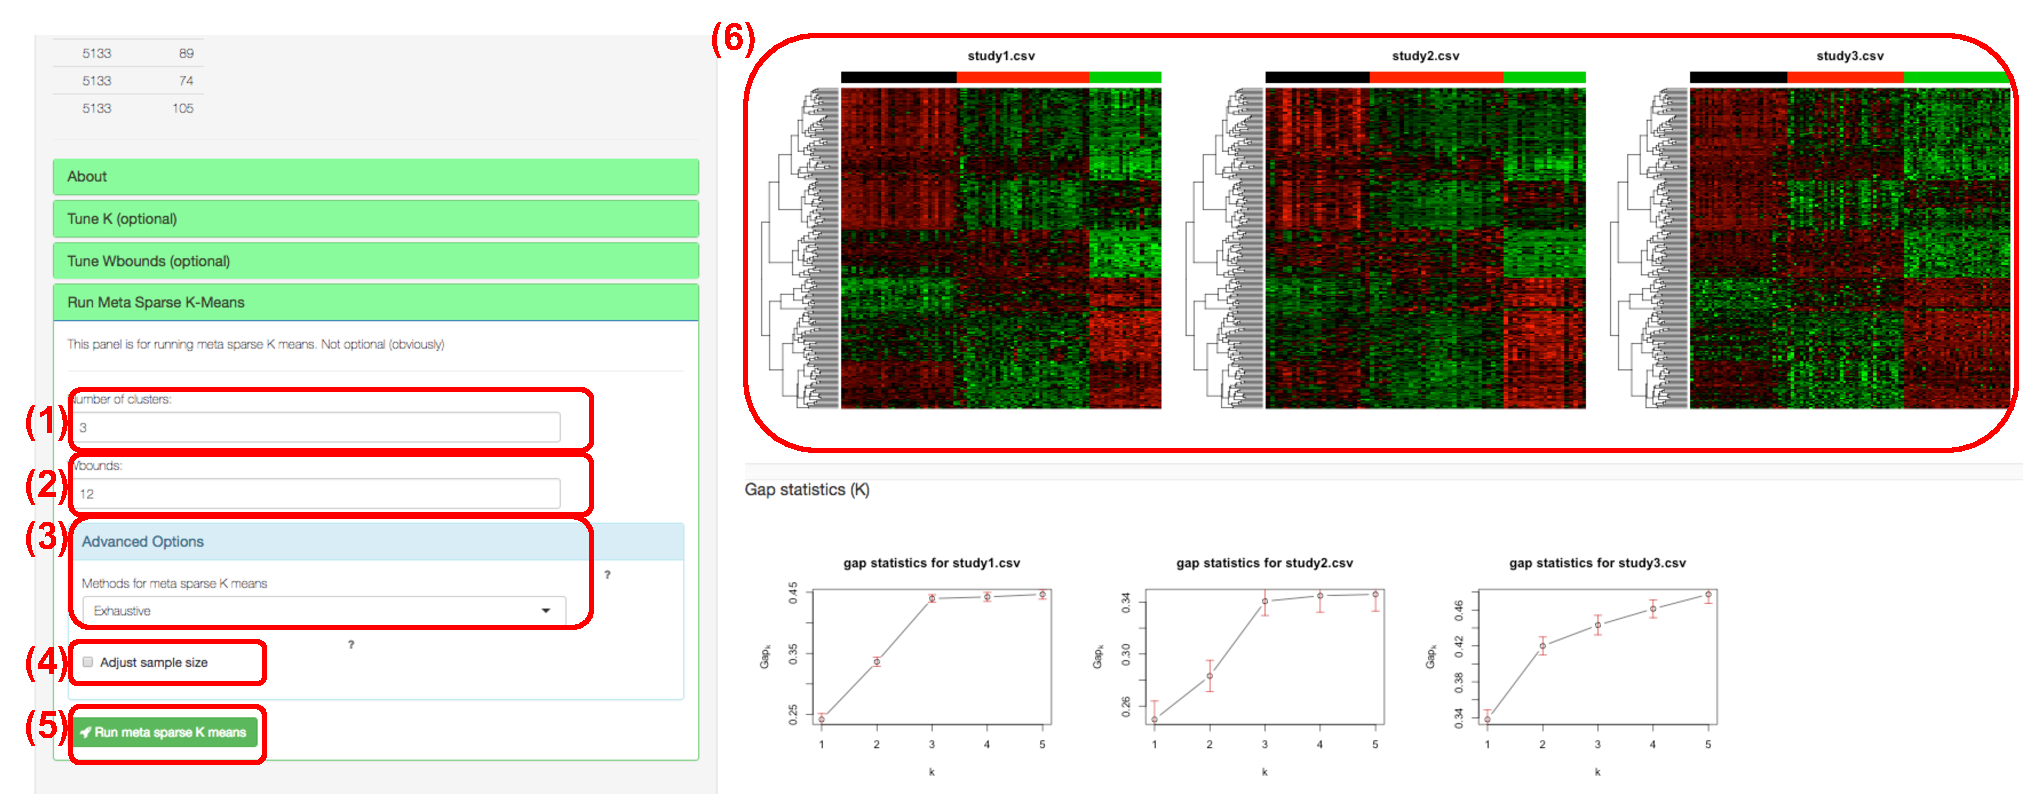
\includegraphics[scale=0.5]{./figure/metaClust/mskmRes.pdf}
\caption{Result for MetaClust}
\label{fig:mskmRes}
\end{center}
\end{figure}
In advanced options (for which users are not suggested to change if they are not familiar with the algorithm), 
There are three clustering matching methods (at position {\color{red} (3)}): Exhaustive, linear, MCMC.
Exhaustive is suggested if the data is not large.
Linear will perform smart search and get solution much faster than Exhaustive, 
but it may yield less accuracy with very low probability.
MCMC is suitable if many studies and clusters are provided.
Adjust sample size checkbox (at position {\color{red} (5)}) allows users to adjust sample size effect.
After number of clusters and Wbounds are specified,
users can click on Run meta sparse K means and obtain results as Figure~\ref{fig:mskmRes}.

\end{steps}

\textbf{Complete List of Options:} 
\begin{enumerate}
\item Tune K (** optional)
\begin{itemize}
\item Maximum of K: the maximum number of K that gap statistics will step through.
\item Top percentage by larger variance: Top percentage p\% by larger variance means that we will use top p\% larger variance genes to perform gap statistics.
\item Number of permutaitons: Number of permutation is number of bootstrap samples for gap statistics.
\item Select studies to be tuned: Studies to be tuned.
\item Tune K: start tuning K.
\end{itemize}
\item Tune Wbounds (** optional)
\begin{itemize}
\item Number of clusters for tuning wbounds: number of clusters for tuning Wbounds.
\item Iterations: Iterations are number of bootstrap samples for gap statistics.
\item Minimum of wbounds: lower bound of the searching space of Wbounds.
\item Maximum of wbounds: upper bound of the searching space of Wbounds.
\item Step of of wbounds: stepsize of the searching space of Wbounds.
\item Tune wbounds: start tuning wbounds.
\end{itemize}
\item Run Meta Sparse $K$-means: 
\begin{itemize}
\item Number of clusters: number of clusters. Can be tuned from Tune K option.
\item Wbounds: control numbers of selected features. Can be tuned from Tune Wbounds option.
\item Methods for meta sparse Kmeans: Exhaustive is suggested if the data is not large.
Linear will perform smart search and get solution much faster than Exhaustive, 
but it may yield less accuracy.
MCMC might by very time consuming.
\item Adjust sample size: adjust sample size effect.
\item Run meta sparse Kmeans: start tuning wbounds.
\end{itemize}

\end{enumerate}


\subsubsection{Results}

We used multi-study leukemia gene expression data as example.
After performing merging of the three datasets, we didn't filter by mean or variance (filter 0\% genes by mean and 0\% by variance) and 5133 genes remained.
In this example actually do not need extra label information.
The result is shown in Figure~\ref{fig:mskmRes} at position {\color{red} (5)}.
We obtained unified feature selection across all studies.
The clusters are well separated in each study and the cluster patterns are consistent across all studies.
The clustering heatmaps and labels are saved in the metaOmics folder.










 
\subsection{MetaPCA}
Dimension reduction is a popular data-mining approach for transcriptomic analysis.
MetaPCA aims to combine multiple omics datasets of identical or similar biological hypothesis and perform simultaneous dimensional reduction in all studies.
The results show improved accuracy, robustness, and better interpretation among all studies.
By clicking the ``Toolsets" tab and then choosing MetaPCA,
users are directed to the MetaPCA homepage, as shown in Figure~\ref{fig:metaPCAHome}.
The R package for the MetaPCA module can be found at \url{https://github.com/metaOmics/metaPCA}.

\begin{figure}[H]
\begin{center}
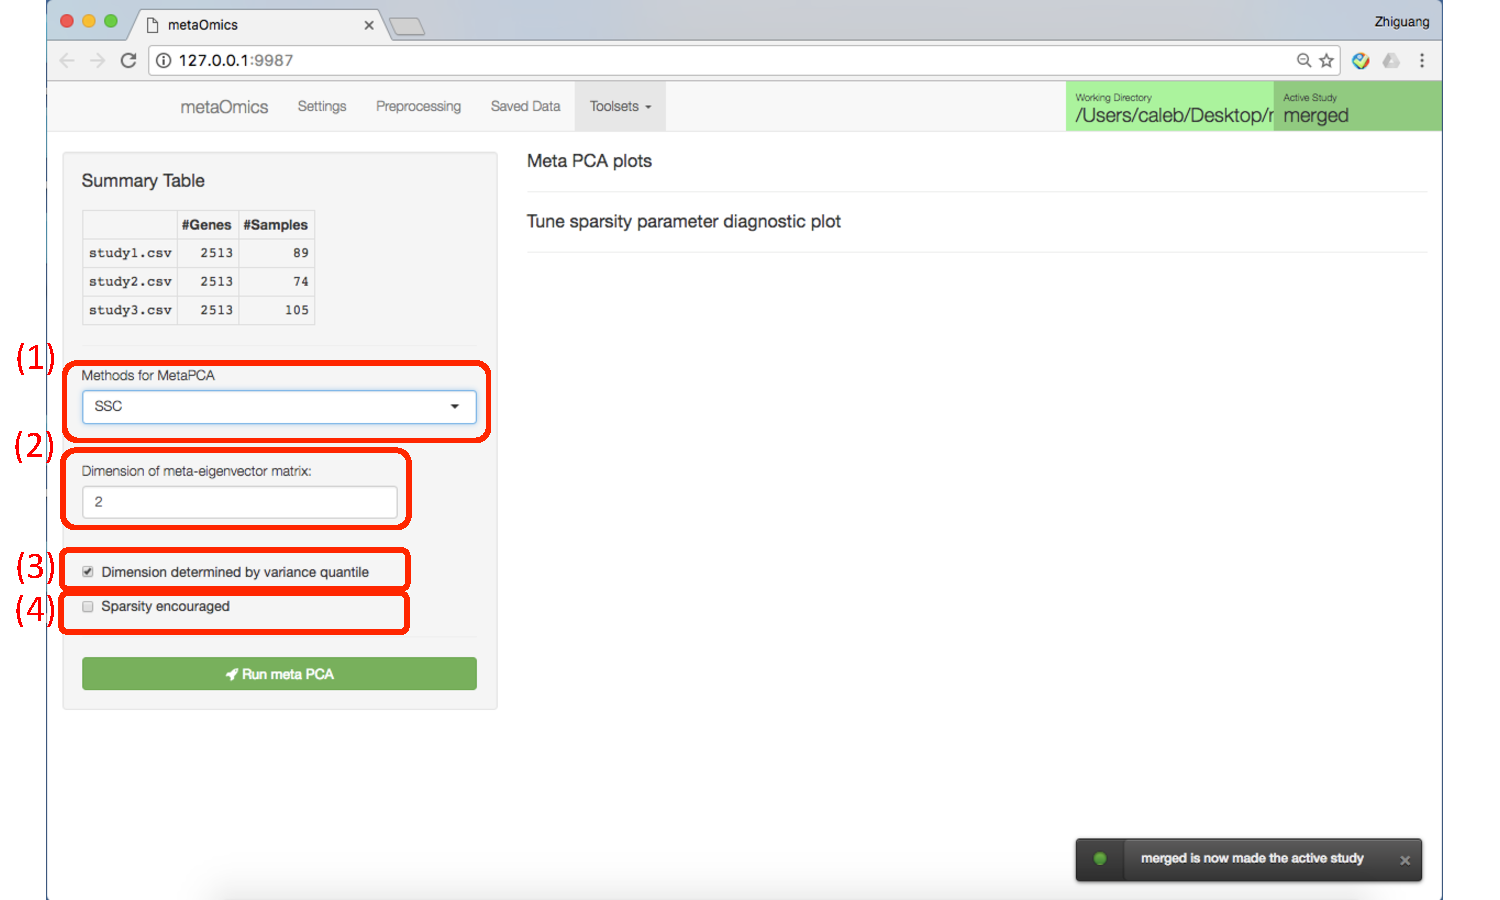
\includegraphics[scale=0.4]{./figure/metaPCA/metaPCAHome.pdf}
\caption{MetaPCA settings}
\label{fig:metaPCAHome}
\end{center}
\end{figure}

\subsubsection{Procedure}

The procedure on describing how to use metaPCA is described below.
A complete list of options is available in Section~\ref{sec:completeList_MetaPCA}.

\begin{steps}

\item \textbf{Specify parameters} 

There are very few parameters that need to be specified for MetaPCA, as in Figure~\ref{fig:metaPCAHome}.
Advanced options are not suggested to be changed unless the users are familiar with the algorithm.
There are two methods for MetaPCA (at position {\color{red} (1)}). 
SSC represents MetaPCA via sum of squared cosine (SSC) maximization.
SV represents MetaPCA via sum of variance decomposition (SV).
Details of SSC and SV can be found in MetaPCA manuscript \citep{kim2017meta}.
SSC has better performance and is suggested.
The dimension of meta-eigenvector matrix option {\color{red} (2)} allows users to specify the dimension of the output meta-eigenvector matrix.
The checkbox of ``dimension determined by variance quantile" is suggested to be checked {\color{red} (3)}.
When checked, the dimension size of each study's eigenvector matrix (SSC) is determined  by the pre-defined level of variance quantile 80\%.
If the checkbox of ``sparsity encouraged" is checked (at position {\color{red} (4)}), users can perform MetaPCA.
After clicking on the ``search for optimal tuning parameter" button, the optimum tuning parameter will be returned to the box ``tuning parameter for sparsity," 
which may be time consuming.

\item \textbf{Perform MetaPCA} 

By clicking the ``Run Meta PCA" button, the MetaPCA module will be performed.


\end{steps}


\subsubsection{Results}
The input dataset is the same as the input for MetaDE module.
%After performing merging of the three datasets and filter 50\% genes by mean and 50\% by variance, 1283 genes remained.
Detailed descriptions of these studies can be found in Table~\ref{tab:realDataLeukemia}. 

The result of MetaPCA is shown in Figure~\ref{fig:metaPCAresult},
which shows nice separations between three groups.
These figures and eigenvectors are saved to the MetaPCA folder.

\begin{figure}[H]
\begin{center}
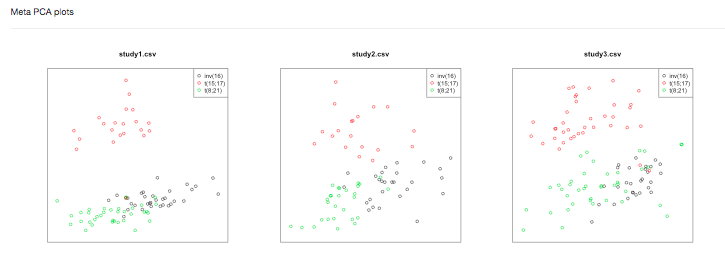
\includegraphics[scale=0.3]{./figure/metaPCA/metaPCA}
\caption{MetaPCA result.
The x-axis (horizontal) is the first principal component, 
and the y-axis (vertical) is the second principal component.
Each dot represents a sample in a study with the sample label marked to the top right of the figure.
}
\label{fig:metaPCAresult}
\end{center}
\end{figure}

 
\subsection{MetaPredict}

Top scoring pairs is a robust algorithm for predicting gene expression profiles,
which adopts nonparametric rank-based prediction rule.
The MetaPredict is a meta-analysis version of the TSP algorithm that combines multiple transcriptomic studies to build a prediction model and shows improved 
prediction accuracy as compared to single study analysis.
The R package for MetaPredict module can be found \url{https://github.com/metaOmic/MetaPredict}.

After opening the MetaPredict page, as shown in Figure \ref{fig:MetaPredictmainpage}, there are 1 drop-down menu (``Methods for MetaPredict") {\color{red} (1)}, three number entries (``Max number of top scoring pairs (K)" {\color{red} (2)}, ``Number of cores for parallel computing" {\color{red} (3)} and ``Number of top scoring pairs (K)" {\color{red} (7)}), three character entries (``Please select TWO labels to cluster" {\color{red} (4)}, ``Please select studies for training" {\color{red} (5)}, and ``Please select studies for testing") {\color{red} (6)} , and two excuting tabs ("Train model" and "Predict"). 

\subsubsection{Procedure}

\begin{figure}[H]
\begin{center}
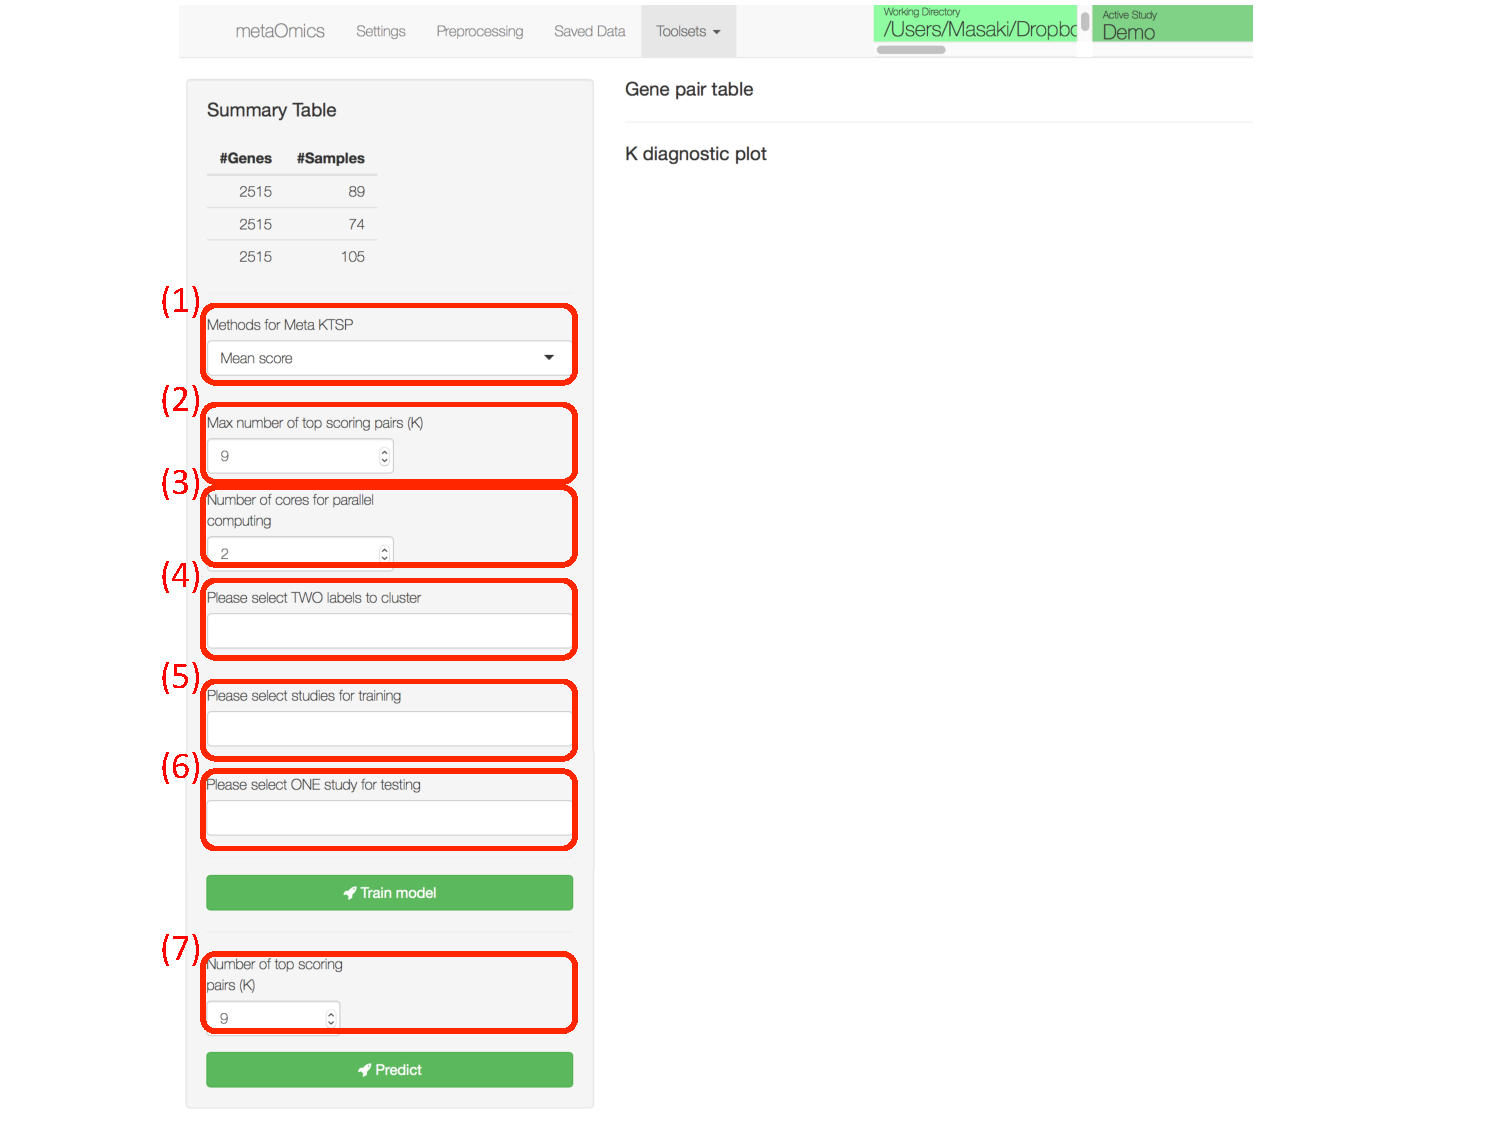
\includegraphics[scale=0.4]{./figure/MetaPredict/MetaPredictprocedure}
\caption{Homepage of MetaPredict}
\label{fig:MetaPredictmainpage}
\end{center}
\end{figure}

\begin{steps}
\item \textbf{Building prediction model based on meta-analysis}

First, we need to decide a method to select K top scoring gene pairs from multiple studies (Figure \ref{fig:MetaPredictmainpage}). 
Second, we need to provide the maximum number of top scoring pairs $K$ (algorithm will search from 1 up to $K$) and the number of cores for parallel computing. 
Next, we need to select only TWO labels to build the classification model. 
In other words, if there exists more than two kinds of labels, we need to choose two from them. 
Our interface will pop up all labels that are available. 
Then, select the dataset as training data and testing respectively, 
and click the "Train model" tab to run the MetaPredict program. 
It may take a while to run the model.

\item \textbf{MetaPredict prediction}

After the model training is finished, on the top right it will show up a ``Gene pair table" ({\color{red} (1)} in Figure \ref{fig:MetaPredictresult}) which present the top $K$ gene pairs statistics. 
A diagnostic plot ({\color{red} (2)} in Figure \ref{fig:MetaPredictresult}) is output to assist users decide which $K$ to use in the final prediction model. 
The suggested value is shown in the plot as green line, which is decided by VO method we introduced in the original paper. Users may also decide $K$ on their own to predict the class label of testing data. 
After deciding $K$, then hit the tab ``Predict'' (Figure \ref{fig:MetaPredictresult}). 
Finally, a confusion matrix is output to show the prediction results ({\color{red} (1)} in Figure \ref{fig:MetaPredictresult}).

\begin{figure}[H]
\begin{center}
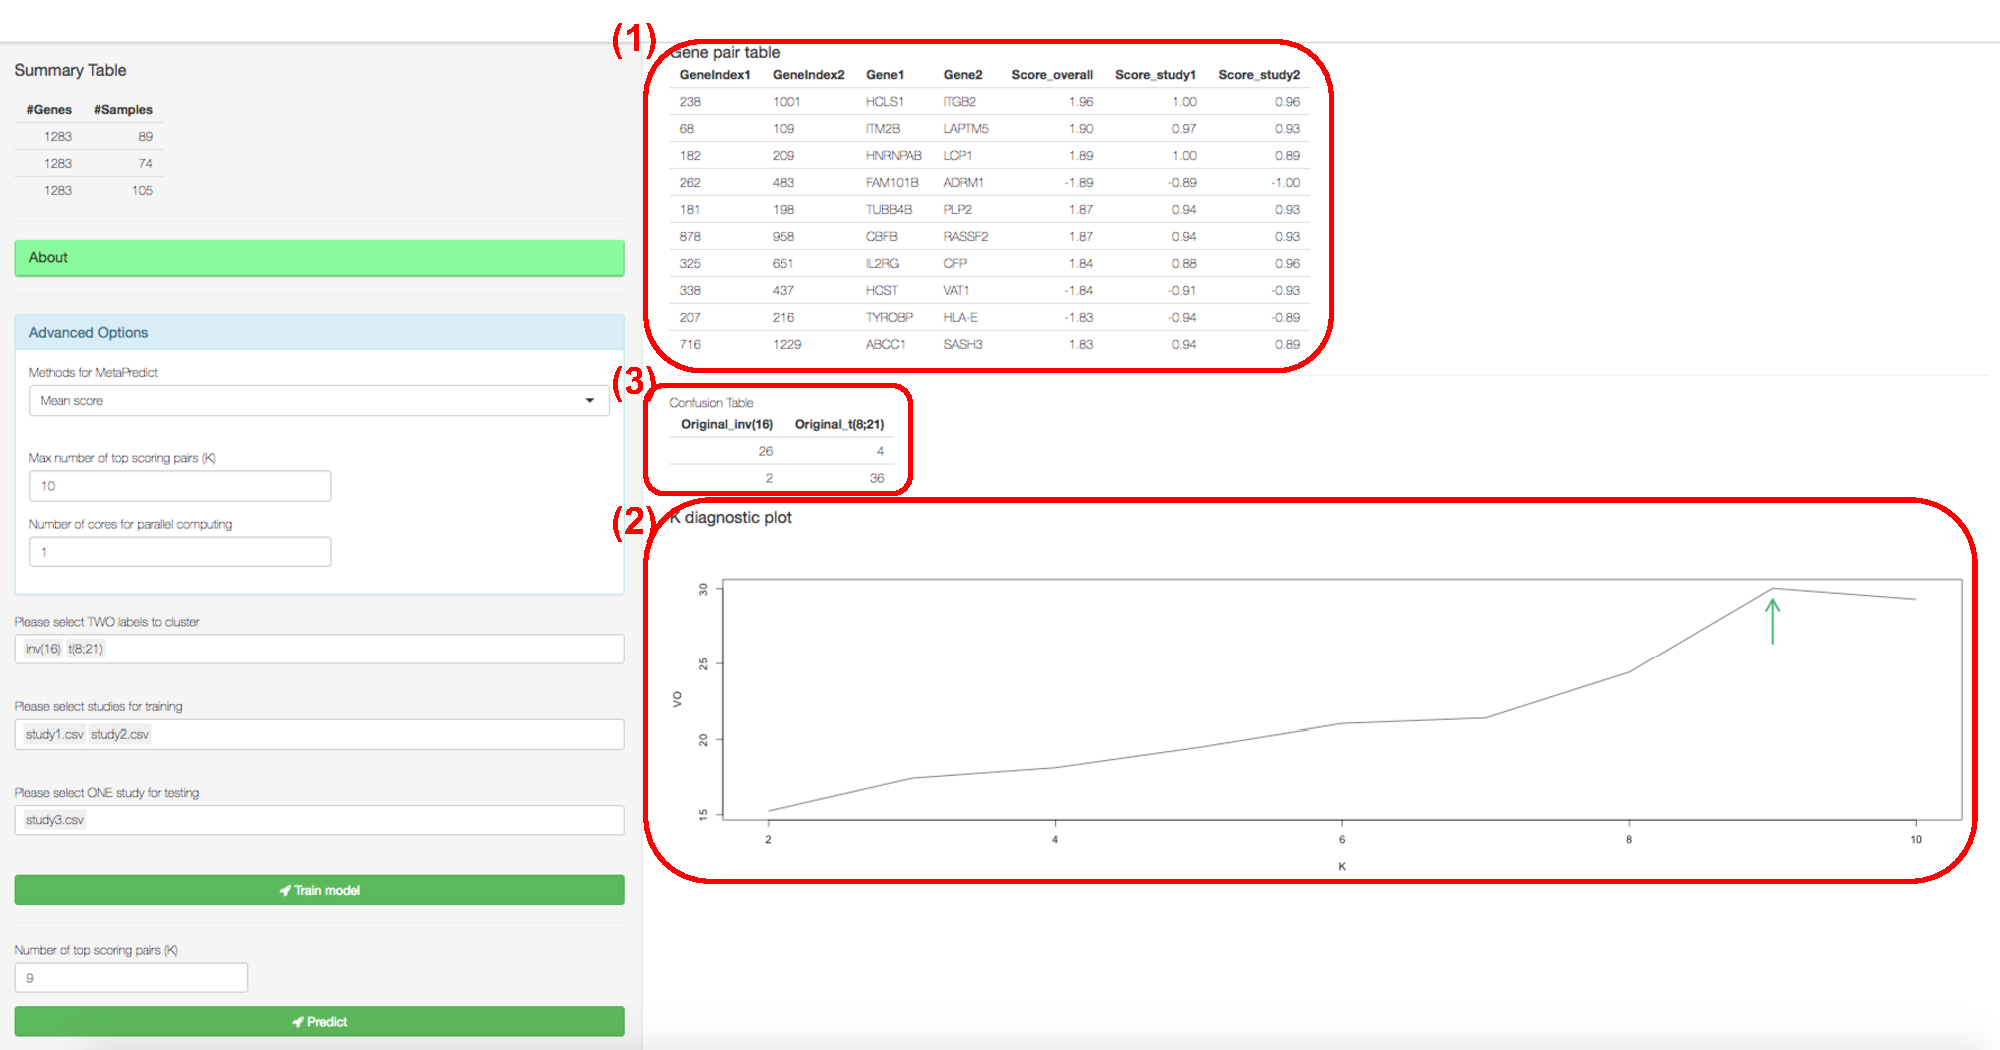
\includegraphics[scale=0.7]{./figure/MetaPredict/MetaPredictresult.pdf}
\caption{Results for MetaPredict.}
\label{fig:MetaPredictresult}
\end{center}
\end{figure}

\end{steps}

\textbf{Complete List of Options:} 
\begin{enumerate}
\item Model trainings: 
\begin{itemize}
\item Methods for MetaPredict: include Mean score, Fisher, Stouffer.
\item Max number of top scoring pairs (K)
\item Number of cores for parallel computing
\item TWO labels to cluster: labels for MetaPredict
\item Please select studies for training
\item Please select studies for testing
\item Number of top scoring pairs (K): Number of top scoring pairs (K) for prediction.
\end{itemize}

\end{enumerate}

\subsubsection{Results}

A confusion matrix is output to show the prediction results ({\color{red} (1)} in Figure \ref{fig:MetaPredictresult}).
The prediction results are also saved in the folder.

 
\subsection{MetaNetwork}
By clicking toolsets and then MetaNetwork,
users are directed to MetaNetwork home page as Figure~\ref{fig:MetaNetworkHome}.
The R package for MetaNetwork module can be found \url{https://github.com/metaOmics/MetaNetwork}.

\begin{figure}[H]
\begin{center}
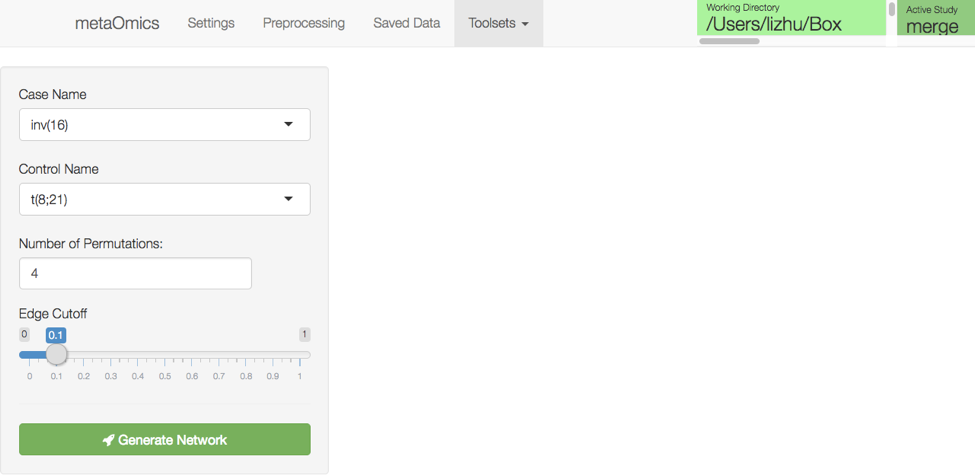
\includegraphics[scale=0.5]{./figure/MetaNetwork/MetaNetworkHome}
\caption{MetaNetwork homepage}
\label{fig:MetaNetworkHome}
\end{center}
\end{figure}

MetaNetwork includes three steps to get differentially co-expressed networks,
including (1) generate network, (2) search for basic modules, and (3) assemble super-modules. 
The left side of Figure~\ref{fig:MetaNetworkHome} is the control panel of step 1. 
The control panel for step 2 and step 3 will show up after the previous step is done.
The explanation of the complete list of all options are in Section~\ref{sec:completeList_MetaNetwork}


\subsubsection{Procedure}

\begin{steps}
\item \textbf{Generate Network}
The first step of MetaNetwork is to generate co-expression network. 
In this step, the network for permuted data will also be generated. 
Users need to select case and control names, the number of permutations, and edge cut-off which determines the proportion of edges to be kept in the network. 
After clicking \textbf{Generate Network} button, screen will show message indicating the algorithm is running to generate network.

\item \textbf{Search for basic modules}

The next step is to search basic modules.
Advanced options (recommended not to change) include the number of repeats used for each initial seed modules (``Number of repeat"),
the maximim Monte Carlo steps for simulated annealing algorithm (MC Steps),
and the maximum pairwise Jaccard index allowed for basic modules (Jaccard Cutoff), as shown in Figure~\ref{fig:MetaNetworkstep2}.
If two repeats from Monte Carlo simulation are very similar (with Jaccard index greater than the cutoff),
only one repeat with stable configuration (low energy) will be kept in the analysis.
Users are suggested to use the default options.
Explanation of these technical terms are omitted in this tutorial,
but readers can refer to \cite{zhu2016metadcn} for details.
After clicking \textbf{Search for basic modules} button in Figure~\ref{fig:MetaNetworkstep2}, 
screen will show message indicating the algorithm is running to search for basic modules.
This step is computationally demanding depending the on gene size.
After this step is done,
the screen will show a table of basic modules highly connected in cases but lose connections in control and vice versa.


\begin{figure}[H]
\begin{center}
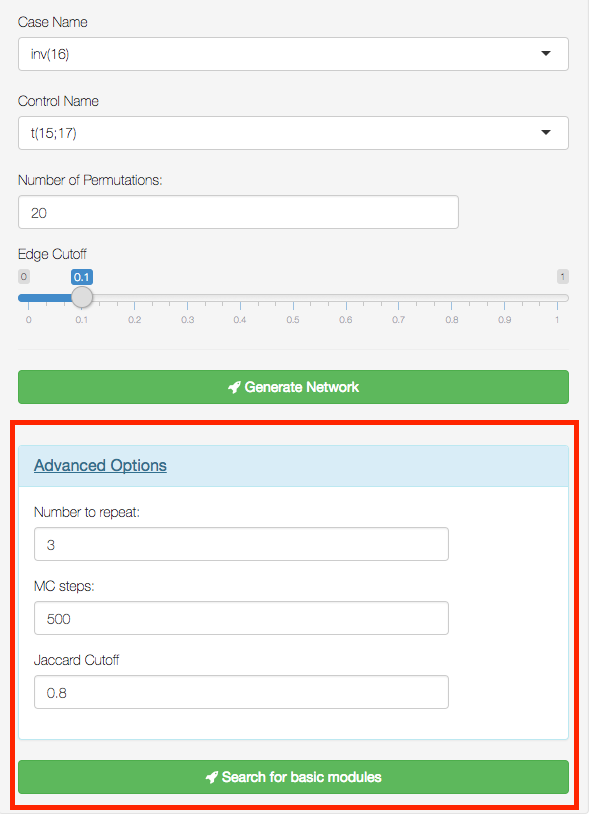
\includegraphics[scale=0.35]{./figure/MetaNetwork/MetaNetworkstep2}
\caption{MetaNetwork control panel for search for basic modules}
\label{fig:MetaNetworkstep2}
\end{center}
\end{figure}

Search for basic modules can be time consuming, 
especially if a large number of genes are used. 
After this step is done, the screen will show a table of basic modules higher correlated in case and a table of basic modules higher correlated in control as in Figure~\ref{fig:MetaNetworkBM}. 

\begin{figure}[H]
\begin{center}
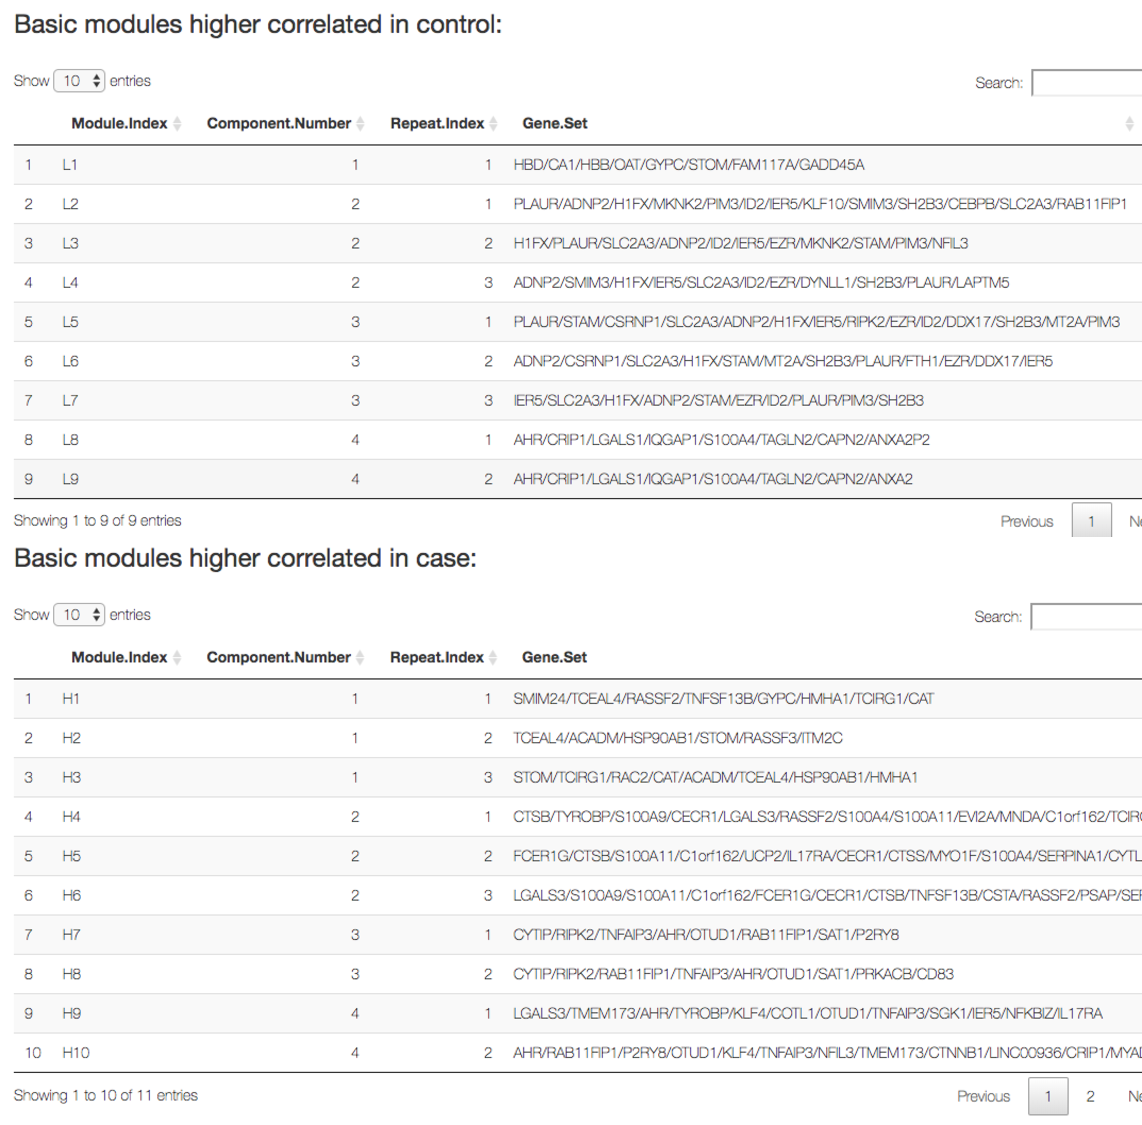
\includegraphics[scale=0.9]{./figure/MetaNetwork/MetaNetworkBM}
\caption{MetaNetwork output from search for basic modules step.
These modules higher correlated in case are labeled as H1, $\ldots$, H6,
and the modules higher correlated in control are labeled as L1, $\ldots$, L6.
The component number and repeat index are for intermediate indexes.
The actual gene sets are listed for each basic module.
}
\label{fig:MetaNetworkBM}
\end{center}
\end{figure}

\item \textbf{Assemble supermodules}

After search for basic modules step is done, the control panel becomes that in Figure~\ref{fig:MetaNetworkstep3}. The last step is to assemble supermodules. Users can decide the FDR cut-off to select basic modules for supermodule assembly. 
After clicking \textbf{Assemble supermodules} button, screen will show message indicating the algorithm is running to assemble supermodules.
A table for basic modules, supermodules and their network visualization will be shown on the right panel of the screen.
MetaNetwork automatically creates files of top supermodules designed to input to a Cytoscape plug-in ``MetaDCNExplorer"
(\url{http://tsenglab.biostat.pitt.edu/software.htm}) for improved visualization and dynamic exploration.

\begin{figure}[H]
\begin{center}
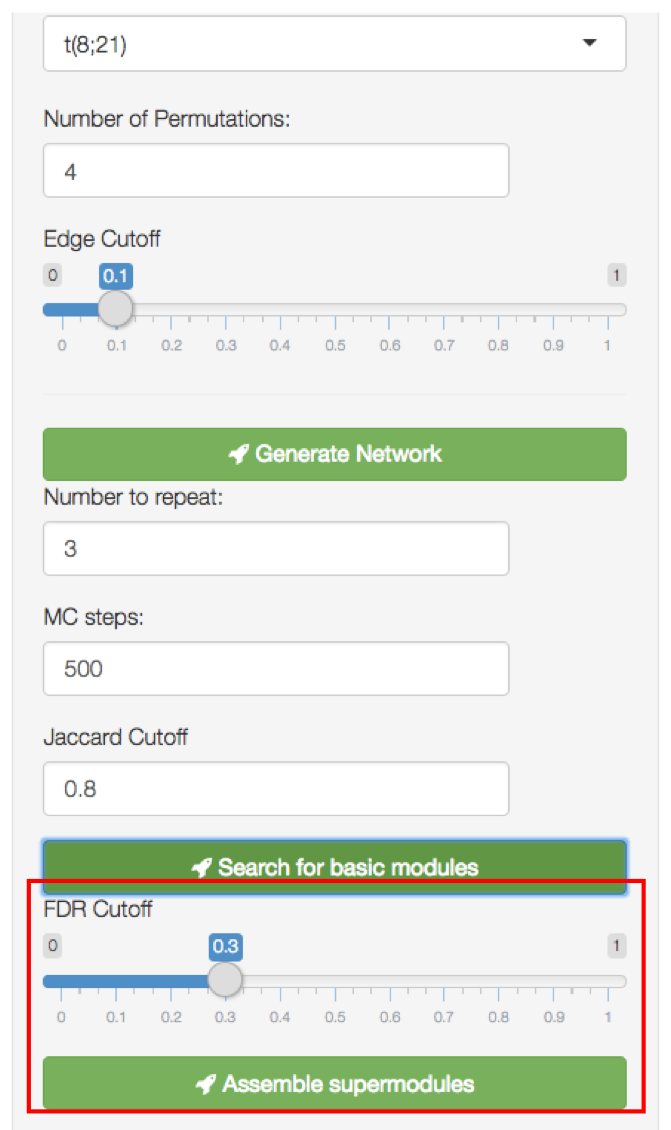
\includegraphics[scale=0.5]{./figure/MetaNetwork/MetaNetworkstep3}
\caption{MetaNetwork control panel for assemble supermodules step}
\label{fig:MetaNetworkstep3}
\end{center}
\end{figure}



\end{steps}

\subsubsection{Results}

We used the leukemia data to demonstrate the MetaNetwork module.
After merging the three datasets by filtering out 80\% of genes by mean and 80\% by variance, 206 genes remained.
In this example we only compare two phenotypes: inv(16) and t(8;21).
Detailed descriptions of these studies can be found in Table~\ref{tab:realDataLeukemia}. 
In general, the MetaNetwork tool is time consuming for large datasets (for both network generation and search for basic modules steps).
We generally suggest users to carefully restrict the number of genes (e.g. less than a thousand) for a test run before implementing large gene set.
By default, all outputs and several interim RData files will be automatically saved to the folder named ``MetaNetwork" under the working directory specified in Section~\ref{sec:setting}.




After the  \textbf{Generate Network} step is done, 
no output will show up in the screen. Instead, a message box will show up indicating several Rdata files are saved in the MetaNetwork folder. 
After \textbf{Search for basic modules} step is done, the screen will show a table of basic modules higher correlated in case or control, 
as in Figure~\ref{fig:MetaNetworkBM}. 
After \textbf{Assemble supermodules} assembly is done, screen will show a table of supermodules (Figure~\ref{fig:MetaNetworksuper}). 
Users can also select basic modules to plot (Figure~\ref{fig:MetaNetworkBMplot}). 
Meanwhile several files will be saved in the MetaNetwork folder.
Detailed explanation of all these intermediate files are described in Section~\ref{sec:completeList_MetaNetwork}.

\begin{figure}[H]
\begin{center}
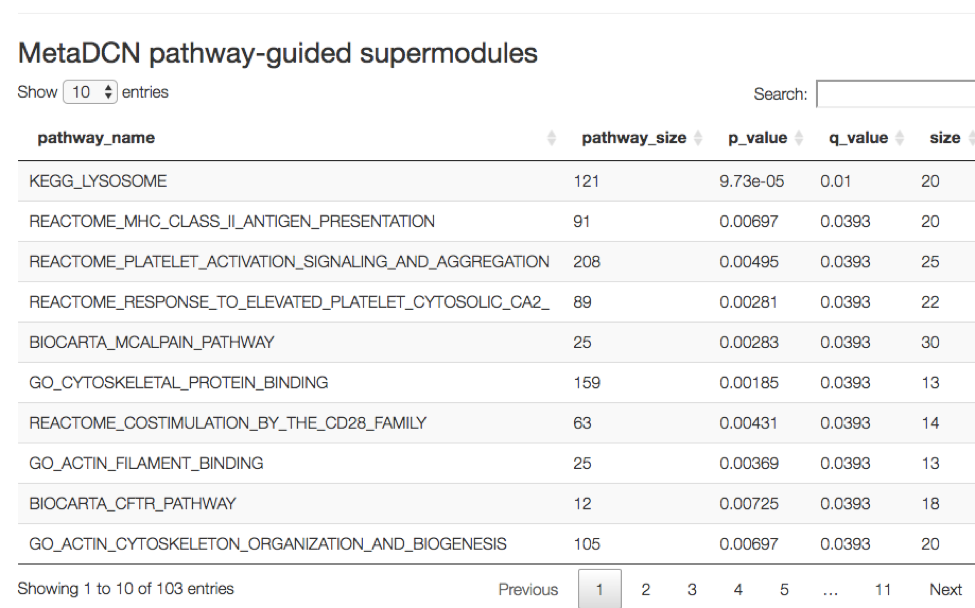
\includegraphics[scale=0.7]{./figure/MetaNetwork/MetaNetworksuper.png}
\caption{MetaNetwork supermodules table.
The second column shows the pathway size.
The third and fourth column show the p-value and q-value of detected supermodule.
The last column is the size of the super module.
}
\label{fig:MetaNetworksuper}
\end{center}
\end{figure}

\begin{figure}[H]
\begin{center}
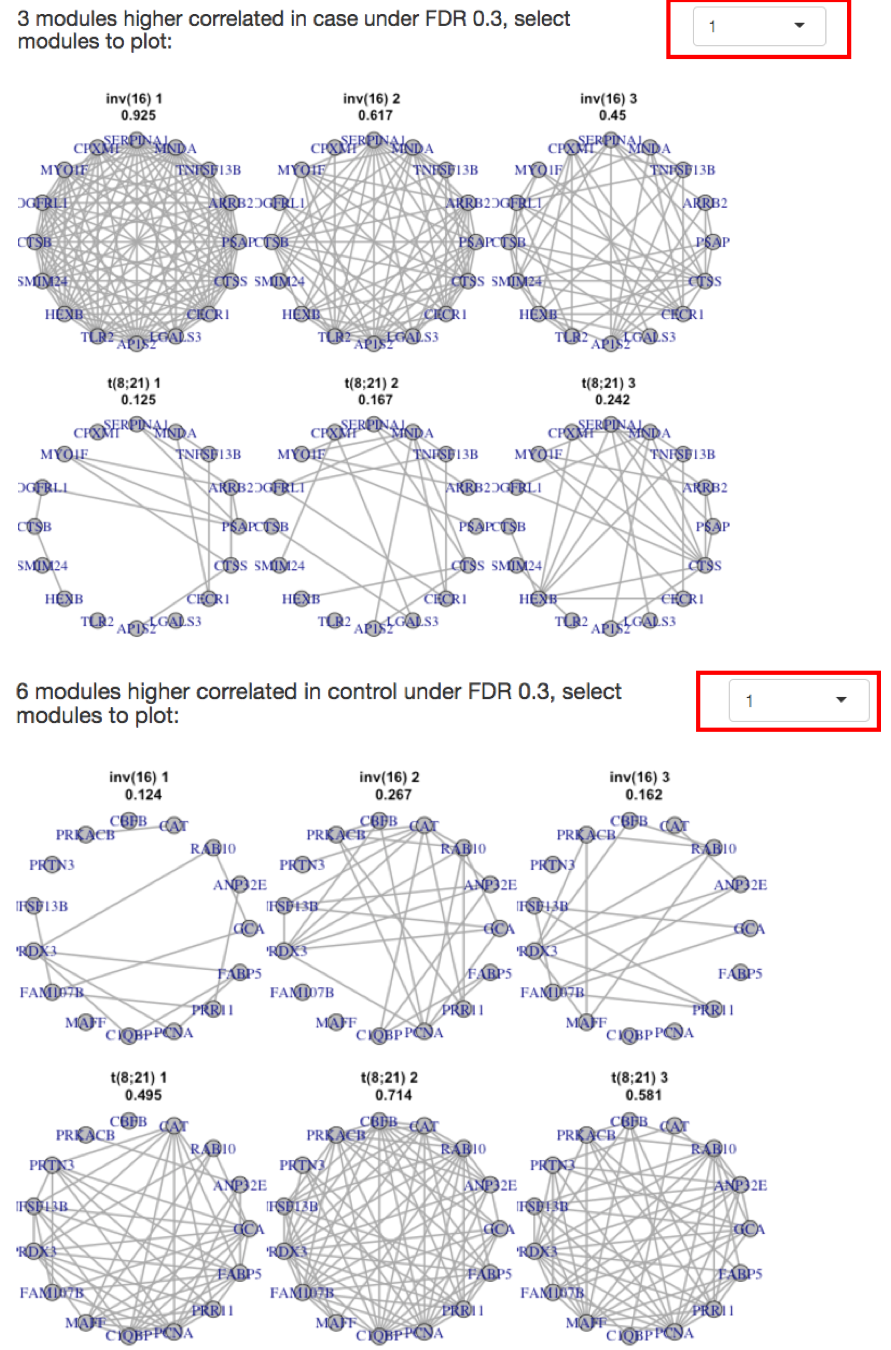
\includegraphics[scale=0.7]{./figure/MetaNetwork/MetaNetworkBMplot.png}
\caption{MetaNetwork select basic modules to plot.
Each dot represents a gene.
An edge represents the two genes are highly correlated.
The network density is marked on top of each network.
The top three modules show higher correlation in inv(16) and the bottom three modules show lower correlation in t(8:21).
}
\label{fig:MetaNetworkBMplot}
\end{center}
\end{figure}
 

%%  for citation purpose
\bibliographystyle{apalike}
\bibliography{reference}
 
\end{document}